\chapter{Split Throughput Heuristic}
\label{sec:splitting}

\begin{figure}[t!]
    \centering
    \begin{subfigure}[b]{\linewidth}
        \centering
        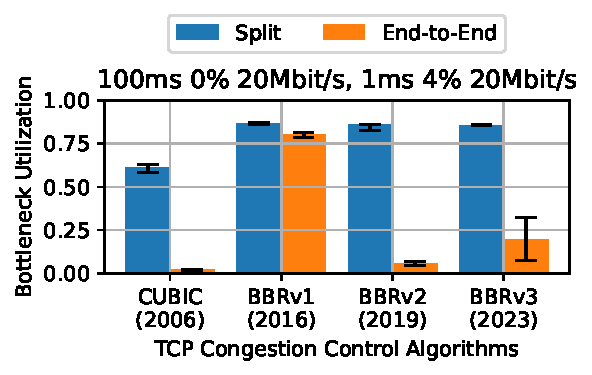
\includegraphics[width=0.8\linewidth]
         {splitting-paper/figures/bbr_over_time/bbr_over_time_network_20_20_100_1_None_None_0_4.pdf}
        \captionsetup{skip=0pt}
        \caption{Asymmetric, lossy last-mile.}
        \label{fig:bbr-over-time:class1}
    \end{subfigure}
    \begin{subfigure}[b]{\linewidth}
        \centering
        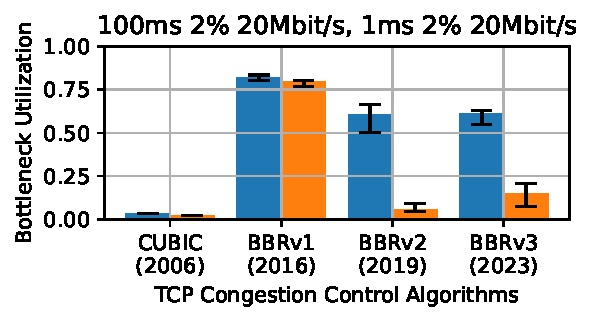
\includegraphics[width=0.8\linewidth]
         {splitting-paper/figures/bbr_over_time/bbr_over_time_network_20_20_100_1_None_None_2_2.pdf}
        \captionsetup{skip=0pt}
        \caption{Asymmetric, both path segments are lossy.}
        \label{fig:bbr-over-time:class2}
    \end{subfigure}
    \begin{subfigure}[b]{\linewidth}
        \centering
        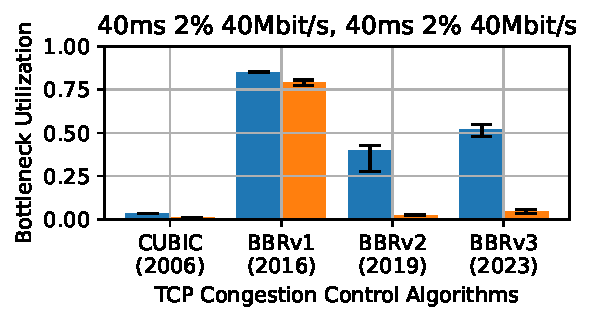
\includegraphics[width=0.8\linewidth]
         {splitting-paper/figures/bbr_over_time/bbr_over_time_network_40_40_40_40_None_None_2_2.pdf}
        \captionsetup{skip=0pt}
        \caption{Symmetric, both path segments are lossy.}
        \label{fig:bbr-over-time:class3}
    \end{subfigure}
    \caption{\small Three classes of network settings in which the throughput of a
     long-lived data transfer using BBRv3 benefits significantly from
     connection-splitting. While the throughput of TCP using BBRv1 may not have
     benefitted from a PEP, as the BBR algorithm has evolved over time, it has
     also made connection-splitting pertinent again. In two of these classes,
     split BBRv3 even achieves high bottleneck link rate utilization where split
     CUBIC does not. IQR of $n=20$.}
    \label{fig:bbr-over-time}
\end{figure}


A stylized history of connection-splitting over the Internet could go
roughly as follows: In the 1970s, TCP was designed as a host-to-host
transport for flow-controlled reliable byte streams. In the late
1980s, TCP implementations added congestion control~\cite{vjk} to
respond to network-path limitations and contention, with indications
of packet loss as the primary congestion signals. As Internet use
exploded in the 1990s, it became apparent that contemporary TCP
implementations performed poorly over long paths with packet loss. By
the late 1990s, many network operators deployed commercial ``TCP
accelerators,'' also known as ``performance-enhancing proxies''
\cite{rfc3135, honda2011still}, to improve customers' TCP
throughput. These proxies transparently split a TCP connection in two,
providing an intermediate point of acknowledgment and retransmission
and transforming an end-to-end TCP connection into two independent
connections.

PEPs were marketed as improving users' throughput, especially where a
PEP splits a high-delay, lossy path into two segments, each with less
delay or less loss. Past surveys found connection-splitting PEPs
deployed on large numbers of wireless and satellite
networks~\cite{rfc3135, honda2011still}. But for almost as long as
these PEPs have existed, purists have criticized their alleged
benefits as exaggerated or unfair, sensitive to the details of an
endpoint's congestion-control scheme, contrary to end-to-end
arguments~\cite{saltzer1984endtoend}, and likely to lead to
ossificiation~\cite{papastergiou2017deossifying, edeline2019bottomup}.

Two more-recent developments have put PEPs on the back foot. The QUIC
transport protocol, standardized in 2021~\cite{rfc9000}, is encrypted
end-to-end and, unlike TCP, its connections can't be split by a
transparent proxy---but its wide deployment by major traffic sources (particularly Google)
in the 2010s didn't produce a measured reduction in performance,
compared with TCP connections that do benefit from PEPs in the
field~\cite{langley2017quic}. If PEPs had really been aiding TCP connections all this time,
QUIC could have been expected to experience lower sustained throughput
over such paths (compared with TCP connections between the same
endpoints, using the same congestion-control schemes).

Furthermore, the BBR congestion-control scheme~\cite{cardwell2017bbr}, first
released in 2016, now controls a large percentage of Internet traffic
(both TCP and QUIC)~\cite{ware2024ccanalyzer} and puts less emphasis on packet
loss as a congestion signal than older schemes in wide
deployment, such as CUBIC. Because much of PEPs' benefit comes from
splitting up long, lossy paths for the benefit of ``loss-based''
schemes, it has been suggested that BBR has led to
a sharp decline in the use of PEPs~\cite{frode}.

\textbf{Do BBR and QUIC make connection-splitting obsolete?} In this
paper, we present findings that suggest that neither of these
developments should be regarded as reliable;
Connection-splitting may yet play a performance-enhancing role
on the Internet, despite its controversial nature.

We conduct a measurement study in emulation to investigate what kinds of
congestion control schemes, network scenarios, and transport protocols may
still experience increased sustained throughput from connection-splitting. We
aid our analysis with a \textit{split throughput heuristic} for predicting the
throughput of a split
connection, based on the measured end-to-end throughput of each segment on the
split path. We aim to (1) explore a wide parameter space of network settings
and congestion control schemes and (2) reason about encrypted transport
protocols (QUIC) that we cannot directly measure.

We present three major findings:

\paragraph{Finding 1: Splitting has become significantly more beneficial to TCP
 BBR since it was initially released in 2016.}

We confirm that BBR's initial ``v1'' release does not benefit markedly from splitting, unlike earlier
congestion-control schemes. But as the BBR algorithm
has evolved into BBRv2 in 2019 and now BBRv3 in 2023, it has also evolved to
behave more conventionally in the sense that it benefits from being
split---just like more traditional, loss-based congestion control schemes such
as CUBIC (\Cref{fig:bbr-over-time}).

The regression in split throughput follows directly from the regression
in end-to-end throughput, via the heuristic. While BBRv1 nearly always achieves
full utilization, BBRv3 sees lower utilization in lossy
settings, leaving more to gain from splitting.
The end-to-end regression is because BBRv3 has increased its loss sensitivity
to coexist fairly with ``loss-based'' schemes such as Reno and
CUBIC~\cite{cardwell2024bbrv3-ietf119,ware2019modeling,zeynali2024promises}.
Thus, we find that BBR and its split behavior continue
to evolve, and that the model-based BBR algorithm has \textit{not} made the
performance enhancements of connection-splitting obsolete.

\paragraph{Finding 2: There exist classes of network paths where TCP BBR would
 significantly benefit from splitting but TCP CUBIC would not.}

Splitting not only benefits BBRv3 in all the same scenarios as CUBIC (in terms
of long-lived throughput), it also benefits BBRv3 in \textit{new} scenarios. In
particular, there exist classes of network settings where the CCA achieves a
very low bottleneck link rate utilization \textit{without} a PEP, but a high
bottleneck link rate utilization \textit{with} a PEP.

More specifically, in addition to edge deployments with a lossy last-mile (\Cref
{fig:bbr-over-time:class1}), BBRv3 can also benefit from splitting in
scenarios where there is loss on both path segments (\Cref
{fig:bbr-over-time:class2}), and when the connection-splitter is located
farther from the edge (\Cref{fig:bbr-over-time:class3}). This suggests that in
these network classes, simple split BBRv3 can replace the
proprietary protocols that have traditionally been used to address middle-mile
loss, particularly in satellite and wireless ad-hoc networks~\cite
{cloudsplitting2010,border2020evaluating,rfc3135}. We should continue to
evaluate the behavior of split CCAs in new types of networks, especially in
space.

\paragraph{Finding 3: Implementations of the ``same'' congestion-control schemes
in QUIC vary significantly, and further differ those of Linux TCP---frustrating
attempts to directly compare performance between QUIC and TCP.}

In an initial study of three QUIC implementations, we find that the end-to-end
behaviors of the same congestion control schemes vary significantly by implementation.
The implementations vary in both baseline performance and sensitivity to loss
and delay. By applying the split throughput heuristic, we find that some
CUBIC implementations can actually benefit in the same classes of network paths
as TCP BBRv3. We also find that BBR is challenging to implement, with various
BBRv3 implementations exhibiting non-uniform end-to-end behavior and thus no
clear trend in split behavior. We argue that the benefits of in-network
assistance should be considered along with not just a CCA, but their specific
implementations. \\

\noindent Our initial evaluation suggests that the performance improvements of
connection-splitting remain relevant in the context of today's model-based
congestion control algorithms, encrypted transport protocols, and satellite and
wireless ad-hoc network settings. As congestion-control schemes continue to
evolve, we urge researchers to refer to them by
algorithm/implementation/version, not just ``BBR'' or even ``QUIC BBRv1''. We
urge the community to create a performance test suite for an implementation to
be able to claim that it conforms to a particular congestion-control standard.
Finally, we hope that this work motivates the community to pursue
protocol-agnostic PEPs that achieve the performance benefits of in-network
assistance without the ossification downsides.

\section{Background: BBR and QUIC}
\label{sec:splitting:background}

In this section, we provide additional context on some concepts that we refer to
throughout the text.

\paragraph{Performance-enhancing proxies.}

The idea of in-network assistance has long brought pain to the hearts of
Internet researchers, protocol designers, and network operators. In particular,
the word ``middleboxes'' is often associated with NATs, firewalls, and other
policy enforcers that modify or inspect data in ways that break end-to-end
behavior. A substantial percentage of Internet paths are affected by feature or
protocol-breaking policies of middleboxes~\cite{edeline2019bottomup}.

In contrast, we refer specifically to the type of assistance provided by
performance-enhancing ``proxies'', or PEPs, that transparently split a TCP
connection in two~\cite{rfc3135}. While PEPs still interfere with end-to-end
transport mechanisms, their goal is to enhance the user experience by
maximizing performance, as opposed to enforce security or routing policies.

Connection-splitting PEPs can enhance performance in several ways. By providing
an intermediate point of acknowledgment and retransmission, PEPs reduce the
length of the feedback loop for signals of loss and congestion. The PEP also
allows each side of the split connection to better optimize congestion control
and flow control for network conditions local to the path segment. We can
expect PEPs to impact a variety of performance metrics, including startup time,
packet jitter, retransmission overheads, and more. In this paper, we focus
only on the impact of connection-splitting on the \textit{sustained throughput}
of long-lived data transfers.

\paragraph{Congestion control.}

Congestion control was originally deployed in the 1980s to manage the explosive
growth of the Internet~\cite{vjk}. Foundational algorithms such as slow start
and fast retransmit eventually became part of the Tahoe congestion control
scheme. Variants such as NewReno and CUBIC emerged over time to improve
performance with fairness~\cite{ha2008cubic}. CUBIC is the default congestion control module for
TCP in the Linux kernel, and widely deployed. It is the primary ``loss-based''
congestion control scheme that we evaluate.

The word ``TCP'' is sometimes used synonomously with the congestion control
algorithms that it implements. In reality, the two are distinct, though deeply
intertwined. For example, the QUIC transport protocol implements many of the
same algorithms as TCP to manage network traffic, even though it runs over UDP~\cite{rfc9000}.
In this paper, we refer to ``TCP'' and ``QUIC'' as the transport protocols,
``Linux TCP'' as the implementation of TCP in the Linux kernel, and congestion
control schemes as the particular manifestations of a congestion control
algorithm in a transport protocol implementation.

\paragraph{BBR.}

Today, the focus on congestion control has shifted towards BBR. BBR is sometimes
referred to as a ``model-based'' congestion control scheme because it relies on
a fundamentally different approach of modeling network bandwidth and round-trip
time. It does not use packet loss as the primary signal for congestion. Google
initially presented BBR in 2016 as addressing the problems of CUBIC in
high-speed networks~\cite{cardwell2016bbr-ietf97}.

Over time, BBR encountered controversy for its unfairness towards loss-based
schemes~\cite{ware2019modeling,philip2021revisiting,cao2019use}. In response,
``v1'' of BBR has now evolved into BBRv2 in 2019 and BBRv3 in 2023, driven by
efforts at Google. Today, Google recommends that BBRv1 and BBRv2 be
deprecated in favor of BBRv3~\cite{cardwell2024bbrv3-ietf119}.

BBR is also widely deployed~\cite
{cardwell2024bbrv3-ietf119-qna,ware2024ccanalyzer}. Google has contributed BBR
implementations to the Linux kernel, and Amazon, Akamai, Meta, and Cloudflare
CDNs all use BBRv1 for TCP. At Google, BBRv3 is used in all google.com and
YouTube public Internet traffic with TCP, and is currently being A/B tested
against BBRv1 in Google QUIC traffic~\cite{cardwell2024bbrv3-ietf119}.
It is estimated that 40\% of traffic used BBR in 2019~\cite{mishra2019great}.

% https://datatracker.ietf.org/doc/draft-cardwell-ccwg-bbr/history/
Since 2017, there have been ongoing efforts to standardize BBR in the IETF~\cite{cardwell2024bbr-ietf-draft}.
However, progress has been slow. The Internet draft goes years or months at a
time without an update at the mercy of Google contributors. While companies
have been quick to adopt BBR in Linux TCP, adoption in QUIC has been slower.
Anecdotally, some have resorted to reverse engineering the Linux
implementation, and some such as Cloudflare, Meta, and Cisco are actively
experimenting with variants of BBRv2+ in their QUIC stacks~\cite
{cardwell2024bbrv3-ietf119-qna}.

\paragraph{QUIC.}

The QUIC transport protocol was originally developed by Google in 2012 to
improve performance for HTTPS traffic and to enable the rapid
evolution of transport mechanisms. QUIC is implemented over UDP, and moves
congestion control development from kernel space to user space.

As of 2021, QUIC is now a standards-track RFC~\cite{rfc9000} with widespread
deployment and interoperability testing~\cite{quic-interop}. It is estimated
that 8.4\% of global websites support QUIC~\cite{w3techs}, many of them major
traffic sources such as Cloudflare.
Still, many high-speed flows remain on TCP due to better TCP hardware
capabilities and ``per-origin'' caching, which complicates multi-CDN
deployments that mix protocols.

Evaluations of QUIC at the Internet scale generally show improved performance
compared to TCP, except in satellite networks. Features like zero-RTT
connection establishment and stream multiplexing enable measured improvements
in search latency, rebuffer rate, and other video playback metrics at
Google~\cite{langley2017quic}. Satellite network operators, on the other hand,
experience strife when it comes to QUIC. Several studies have measured the
negative impact of encryption on performance in split satellite
environments~\cite
{kosek2022quicpep,martin2022suitability,kuhn2021quic-over-sat,border2020evaluating}.

\section{Split Throughput Heuristic}
\label{sec:splitting:heuristic}

When initially considering which network scenarios to evaluate in our emulation
study, we discovered it to be non-trivial to pick scenarios that would lead to
a general understanding of the throughput of a congestion control scheme in a
split setting. It is challenging to select which network settings and
combinations of path segments to evaluate, as the parameter space for
combinations of path segments can be quite large. Also, not all CCA
implementations can be trivially split.

For this paper, we refer to \textit{throughput} as the throughput of a
long-lived data transfer in an emulated network, using a single flow.
We do not evaluate other metrics such as startup time, retransmission
overheads, or short-lived data transfers, which have been of interest to
PEPs and could also be impacted by connection-splitting.
When discussing throughput, we refer to \textit{end-to-end throughput} as
the throughput of an end-to-end connection, and \textit{split throughput} as the
throughput of the same connection when there is a connection-splitting PEP.

We realized that while split throughput is not necessarily well
understood for any combination of CCA, transport protocol, and network setting,
the end-to-end throughput often \textit{is}. We make the following insight
based on an ideal setting:

\begin{figure}[h]
  \centering
  \begin{tcolorbox}[colback=yellow!20, width=\linewidth, sharp corners]
    \textbf{Split Throughput Heuristic:} We can estimate the long-lived ``split
     throughput'' of a connection by measuring the long-lived ``end-to-end
     throughput'' on each segment of the split path and taking the minimum.
  \end{tcolorbox}
  \caption{A heuristic for evaluating split behavior from end-to-end behavior in
   an emulated network.}
  \label{fig:heuristic}
\end{figure}

\noindent Thus if we know the throughput of the much smaller parameter
 space of end-to-end connections, we can easily derive:

\begin{enumerate}[noitemsep]
    \item The split throughput of a CCA on a network path composed of two path
     segments,
    \item The end-to-end throughput on the network path,
    \item The expected throughput benefit of using a connection-splitting PEP
     on the network path.
\end{enumerate}

Furthermore, it is impossible to quantitatively evaluate the split throughput
of encrypted transport protocols without creating a custom and explicit
connection-splitting PEP. As a result, it is challenging to establish a
baseline for the throughput that is potentially achievable by QUIC with
in-network assistance, leaving many studies to compare QUIC only to split TCP~\cite
{thomas2019google,border2020evaluating,yuan2024sidekick}. The split throughput
heuristic allows us to estimate the throughput of encrypted transport
protocols using knowledge about its end-to-end throughput, without
actually splitting the connection.

In \Cref{sec:splitting:accuracy}, we discuss potential sources of error in the heuristic,
including the lack of consideration of the queue configuration on the proxy
or the placement of the bottleneck link relative to the data sender. However,
we believe there is a design tradeoff in accuracy versus simplicity.

In the rest of this section, we first describe how to use this heuristic to
analyze the split throughput benefit in a single network setting, without
having to run an emulation with a connection splitter. Then we describe how we
cache emulation results for an end-to-end parameter space to enable a more
open-ended analysis of CCAs over a variety of networks. Finally, we discuss the
limitations of our methodology using the heuristic, and propose possible
extensions.

\subsection{Example Usage in a Single Network Setting}
\label{sec:splitting:heuristic:example}

\begin{lstfloat}[t]
\begin{lstlisting}[language=Python]
class NetworkModel:
    def __init__(self, delay, bw, loss):
        self.delay = delay
        self.bw = bw
        self.loss = loss

def compose(s1: NetworkModel,
            s2: NetworkModel) -> NetworkModel:
    delay = s1.delay + s2.delay
    bw = min(s1.bw, s2.bw)
    loss = s1.loss * (1-s1.loss)*s2.loss
    return NetworkModel(delay, bw, loss)

def throughput(s: NetworkModel) -> float:
    return run_emulation(s)
\end{lstlisting}
\captionof{lstlisting}{An interface for modeling a network path and estimating
 throughput. The \texttt{compose()} function models an end-to-end network path
 from two path segments. The \texttt{throughput()} function obtains a throughput
 measurement for a path segment.}
\label{lst:multi-segment-network-model}
\end{lstfloat}

\begin{lstfloat}[t]
\begin{lstlisting}[language=Python]
def pred_split_throughput(s1: NetworkModel,
                          s2: NetworkModel) -> float:
    return min(throughput(s1), throughput(s2))

def pred_e2e_throughput(s1: NetworkModel,
                        s2: NetworkModel) -> float:
    s = compose(s1, s2)
    return throughput(s)
\end{lstlisting}
\captionof{lstlisting}{Functions that apply our simplified network model and the
 split throughput heuristic (\Cref{fig:heuristic}) to predict split and
 end-to-end throughput, using the interface in \Cref
 {lst:multi-segment-network-model}.}
\label{lst:pred-throughput-api}
\end{lstfloat}

Given a network model of the two path segments that compose an end-to-end
network path, we would like to be able to estimate the expected throughput
benefit of using a connection-splitting PEP between the two segments. In our
emulation study, our simplified network model consists of three
parameters: delay, bandwidth, and loss.

We explicitly define the interface we
use to query split and end-to-end throughput in \Cref
{lst:multi-segment-network-model,lst:pred-throughput-api}. In addition
to the network model, we implement functions to \texttt{compose()} a model of
an end-to-end network path from two path segments and to
query the end-to-end \texttt{throughput()} of a segment.

\paragraph{The \texttt{compose()} function.}
Since our network model consists of three parameters, we describe how to compose
each of these parameters to model the end-to-end network path. Bandwidth is the
minimum of the two bandwidths, which is the bottleneck.
(We may also refer to ``bandwidth'' as ``link rate.'')
Delay is just additive.
If we think of loss as independent random loss, then the composition
of the two is $loss = loss1 + (1-loss1)\cdot loss2 = loss1 + loss2 -
loss1 \cdot loss2$.

Note that many combinations of path segments can compose to the same end-to-end
network path. This makes sense because regardless of where on the network path
loss occurs or which path segment has the bottleneck bandwidth, from an
end-to-end perspective, the network properties look the same.

\paragraph{The \texttt{throughput()} function.}
This is the throughput of a long-running HTTPS connection in a
\texttt{mininet} emulation. The emulated network is parameterized
by the network model of a single path segment, and the HTTPS implementation
uses the congestion control scheme of interest. We describe additional details
about the emulation in \Cref{sec:splitting:methodology}.

\paragraph{Calculating the split improvement.}

\Cref{lst:pred-throughput-api} demonstrates how we can estimate the split
throughput benefit using the interface in \Cref
{lst:multi-segment-network-model}. We \texttt{pred\_split\_throughput()} by taking
the minimum measured throughput on each network path segment, and \texttt
{pred\_e2e\_throughput()} by composing the path segments into an end-to-end
network path and using the measured throughput of that network path. The split
throughput benefit is just how much the split throughput has improved (if it has)
relative to the end-to-end throughput.

\subsection{Caching Throughput Measurements}
\label{sec:splitting:heuristic:caching}

While we can now predict split throughput for congestion control schemes which
are not easily
splittable, evaluating split throughput on a variety of network settings still
requires running emulations for each query. In order to speed up our analysis,
we select a parameter space of delay, bandwidth, and loss within our network
model and cache the end-to-end emulation results for this parameter space. We
describe our choice of parameter space and other modifications as follows:

\paragraph{Selecting a parameter space.} 
\begin{table}[t!]
  \centering
\begin{tabular}{ l l l l l }
  \toprule
    \textbf{Parameter} & \textbf{Values} & \textbf{Unit}\\
    \midrule
    Bandwidth & [10, 20, 30, 40, 50] & Mbit/s \\
    Delay & [1, 20, 40, 60, 80, 100] & ms \\
    Loss & [0, 1, 2, 3, 4] & \% \\
\bottomrule
\end{tabular}
  \caption{\small \label{tab:parameters} Network parameter space for the $5 \cdot
   6 \cdot 5 = 150$ combinations of network settings that we
   analyze in \Cref{sec:results}. These values attempt to realistically
   reflect network settings in which we'd see a PEP.}
   \vspace{-0.4cm}
\end{table}


We select a range of values we thought would realistically reflect network
settings in which we'd see a PEP (\Cref{tab:parameters}). We select propagation
delays from $1$ ms for a Wi-Fi last hop to $100$ ms to reflect the longer RTTs
of a satellite connection. Bottleneck bandwidths range from $10$ to $50$ Mbit/s
for a single connection, and are within the CPU constraints of emulation. Random
loss rates range from $0\%$ for a stable connection to $4\%$ for random loss
caused by e.g., wireless interference and extraterrestrial weather.

\paragraph{Modifying the \texttt{compose()} function.}
We make some subtle changes to the compose function to keep composed network
models within our parameter space.
In some sense, each parameter e.g., delay, can be thought of as an algebraic
group where the operator function is defined in \texttt{compose()}.

For path segments with small delays (1 ms),
we consider the composed path segment to
just have the delay of the longer segment, so we can have segments
with $1$ ms delay. For loss, note that when loss rates are small, $loss1 \cdot
loss2$ is negligibly small. In our case, the loss is always below $4\%$, so we
omit the term in the composition and loss becomes additive.

\paragraph{Collecting data efficiently.}
For some CCAs, we expect a large number of network settings in the parameter
space to have extremely low throughput. Thus we set a utilization threshold of
$5\%$ of the link rate below which we are not interested in the exact throughput
of that network setting.

To more efficiently build the cache, we run a search algorithm on
the parameter space to explore faster network settings first.
The initial network setting we evaluate has the lowest delay, bandwidth, and
loss. We explore adjacent data points if and only if the current data point has
not timed out.

\subsection{Limitations}
\label{sec:splitting:heuristic:limitations}

Although our methodology is more efficient for evaluating many network
settings and enables the exploration of theoretical scenarios,
caching measurements in emulation still takes non-negligible time. A much faster
method to estimate sustained throughput would be to use a theoretical model, such as the
TCP macroscopic model for AIMD schemes~\cite{mathis1997macroscopic}.
However, this method does not reflect the nuances of implementation, and as
Mathis states himself, new models are needed for BBR and modern paradigms~\cite
{mathis2019deprecating,mathis2008reflections}.

Another limitation is our simplified network model and emulation testbed.
One could incorporate more parameters into the network model, such as the
fluctuating bandwidths of cellular networks~\cite{hayes2019mmwave}, or how BBR
incorporates ACK aggregation~\cite{cardwell2018bbr-ietf101}. Another idea is to
generate end-to-end measurements from real testbeds instead of emulation. We
believe these challenges are not limited to emulation studies on split
performance, and hope to use the much more well-understood space of end-to-end
behavior to extrapolate split behavior.

We acknowledge that we only test connections in a single-flow environment.
This limits what we can say about inter-flow fairness, but we can still infer
some aspects from how congestion-control schemes respond to loss and delay in
isolation, a classical concept known as ``TCP friendliness''~\cite{rfc5348}.
While split connections reduce retransmissions by buffering on the path,
their high throughput may also make them unfair. There may also be different
fairness implications when combining split with end-to-end connections.
If every connection is split, then we refer to other studies for understanding
fairness at scale for each side of the concatenation~\cite
{philip2021revisiting}.

We also acknowledge that TCP is not limited to bulk data transfers, and that
it would be valuable to study other metrics that could be impacted by
connection-splitting, such as startup time, packet jitter, and retransmission
overheads.

Finally, our heuristic makes the simplified assumption that we can identify the
bottleneck path segment based on the minimum measured throughput. In reality,
the ability of a data sender to sustain that throughput depends on its ability
to saturate the send buffer. This is particularly true for data senders farther
along the network path, as their behavior will depend on the queue
configuration and the burstiness of previous senders. We explore this more
in \Cref{sec:splitting:accuracy}.

\section{Methodology}
\label{sec:splitting:methodology}

\begin{figure}[t]
    \centering
    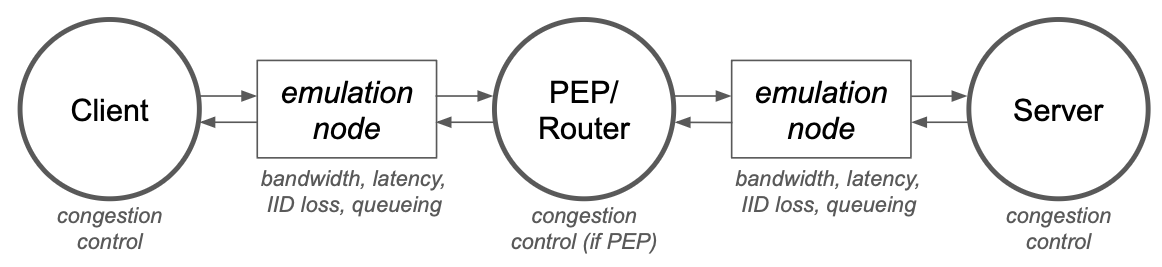
\includegraphics[width=\linewidth]{splitting-paper/figures/mininet-topology.png}
    \caption{Two-segment network topology in \texttt{mininet}. The
     middle node splits the path into two segments with different properties.}
    \label{fig:mininet}
\end{figure}

\begin{table}[t!]
  \centering
\footnotesize
\begin{tabular}{ l l l l l }
  \toprule
    \textbf{CCA} & \textbf{Implementation}\\
    \midrule
    BBRv3 & Linux TCP v6.4.0+ \texttt{google-bbr/v3} fork\\
    BBRv2 & Linux TCP v6.4.0+ \texttt{google-bbr/v2alpha} fork\\
    BBRv1 & Linux TCP v5.15.0-122-generic \\
    CUBIC & Linux TCP v5.15.0-122-generic \\
    % TCP & BBRv1 & Ubuntu 22.04.2 with Linux kernel 6.1, 6.8; Ubuntu 18.04.1 with Linux kernel\\
    % & & 4.15, 4.16, 4.17, 4.18, 5.0, 5.4, 5.19; Ubuntu 18.04.1 with Linux kernel v4.9,\\
    % & & 4.10, 4.11, 4.12, 4.14 (Docker Ubuntu 16.04 for build)\\
    BBRv3 & Google \texttt{quiche} v131.0.6728.1 \\
    BBRv1 & Google \texttt{quiche} v131.0.6728.1 \\
    CUBIC & Google \texttt{quiche} v131.0.6728.1 \\
    BBRv2 & Cloudflare \texttt{quiche} v0.14 \\
    BBRv1 & Cloudflare \texttt{quiche} v0.14 \\
    CUBIC & Cloudflare \texttt{quiche} v0.14 \\
    BBRv2 & IETF \texttt{picoquic} \texttt{29c7c53} \\
    BBRv1 & IETF \texttt{picoquic} \texttt{29c7c53} \\
    CUBIC & IETF \texttt{picoquic} \texttt{29c7c53} \\
\bottomrule
\end{tabular}
  \caption{\small \label{tab:cca-implementations} The congestion control schemes and
   transport protocol implementations we evaluate in the measurement study.}
  \vspace{-0.4cm}
\end{table}


We want to evaluate different congestion control schemes in a variety of network
settings. To do this, we run emulation experiments in \texttt{mininet} with
simple HTTPS clients and servers to measure the throughputs of long-lived data
transfers. In this section,
we describe our emulated network configurations, HTTPS endpoints and
PEP, and other specifications.

\paragraph{Network configuration.}

We used two linear network topologies: a one-segment topology for caching
end-to-end measurements and a two-segment topology for evaluation with a
connection-splitting PEP (\Cref{fig:mininet}). Both have
a client and server node at each end. The two-segment topology additionally has
a router node in between. Each path segment has a bridging node to emulate network
properties on the link.

We parameterize each path segment in three dimensions: delay, bandwidth, and a
random loss rate. We configure the network properties on the bridging nodes'
egress interfaces, using \texttt{tc-netem} to set delay and random loss,
and \texttt{tc-htb} to set bandwidth. Additionally, we use \texttt{tc-qdisc} to
configure the queues to use RED\footnote{We apply RED and not droptail because it gives more
continuous feedback about loss for congestion control, and is commonly used in
core routers. We also do not need the multi-flow and low-delay properties of
other queue disciplines. We use RED in \texttt{adaptive harddrop} mode with a
maximum queuing delay of $\approx1$ BDP. Exact parameters are available in the code.},
which is the source of congestive loss.
Each link is symmetric in
the uplink and downlink directions. For some versions of BBR, we set an \texttt
{fq} qdisc on the host nodes' egress interfaces for pacing.

\paragraph{Host configuration.}

We create simple HTTPS wrappers around each transport protocol implementation to
evaluate the congestion control schemes in \Cref{tab:cca-implementations}. The TCP
endpoints use the Python \texttt{http} module. For the QUIC implementations, we
modify comparable client/server applications from each repository.
%to transfer some number of bytes from server to client.
With the exception of enabling TCP pacing where required by BBR, we use
``default values'' for tunable parameters, considering these to be part of each
implementation.

In TCP, we set the CCA by using a specific Linux kernel
version and loading the congestion control module. We use the default
kernel's implementations of CUBIC and BBRv1, and Google's kernel fork for
BBRv2 and BBRv3 (\Cref{tab:cca-implementations}).

In QUIC, we simply select the CCA as a command-line
argument to the user space implementation. We evaluate Google \texttt
{quiche}~\cite{google-quiche}, Cloudflare \texttt{quiche}~\cite
{quiche}, and \texttt{picoquic}~\cite{picoquic}. Google and Cloudflare \texttt
{quiche} are their production implementations of the same name,
and \texttt{picoquic} is a minimalist implementation based on the IETF spec.
All three include CUBIC and BBRv1 implementations, as well as some form of
BBRv2 or BBRv3, which is still undergoing standardization.

For the transparent, connection-splitting TCP PEP, we use PEPsal~\cite
{caini2006pepsal}. PEPsal intercepts the SYN packet during the three-way
handshake and forms separate TCP connections with each endpoint,
copying data between the two sockets. Note that
discussions of split QUIC are based only on the split throughput heuristic
and do not use an actual splitter.

\paragraph{Experiment specification.}
In each experiment, the HTTPS client requests a specific number of bytes to be
transferred from the server in the HTTPS payload. This number corresponds to the
amount of data that can be transmitted through the bottleneck link over a
$10$-second period. We have found this to be sufficiently large to reflect
sustained throughput.

In practice, we report the "single-stream goodput" calculated as the number of
application-layer bytes received (excluding HTTPS headers) divided by request
completion time (from when the client sends a request to when it receives a
complete response). Due to header overhead and request latency, this metric
will never equal the link rate.

\paragraph{Machine specification.} All experiments use CloudLab~\cite
 {duplyakin2019design} x86\_64 rs630 nodes in the Massachusetts cluster running
 Ubuntu 22.04.2. The nodes use the default Linux kernel v5.15.0-122-generic,
 except for TCP BBRv2 and BBRv3.%, in which they use the Google fork of v6.4.0+.

\section{Measurement Study Results}
\label{sec:splitting:results}

\begin{figure*}[t!]
    \centering
    \begin{subfigure}[b]{0.22\linewidth}
        \centering
        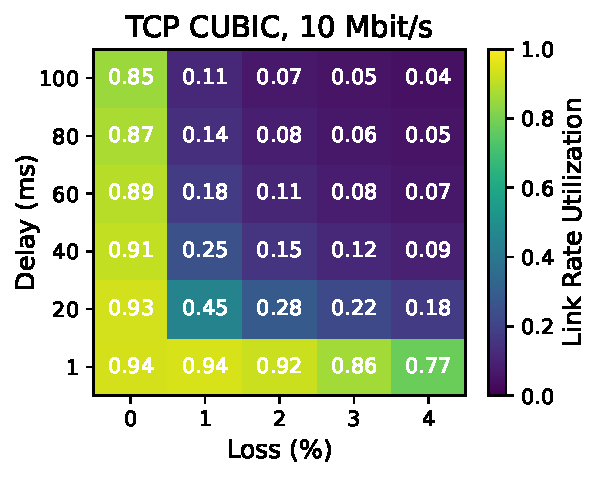
\includegraphics[width=\linewidth,trim={0 0 2cm 0.7cm},clip]
         {splitting-paper/figures/heatmaps/heatmap_tcp_cubic_10mbps.pdf}
        \captionsetup{skip=4pt}
        \caption{TCP CUBIC.}
        \label{fig:2d-heatmap:cubic-10}
    \end{subfigure}
    \begin{subfigure}[b]{0.22\linewidth}
        \centering
        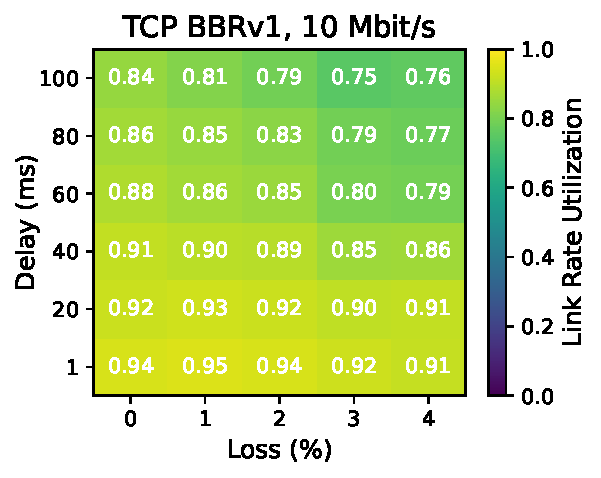
\includegraphics[width=\linewidth,trim={0 0 2cm 0.7cm},clip]
         {splitting-paper/figures/heatmaps/heatmap_tcp_bbr1_10mbps.pdf}
        \captionsetup{skip=4pt}
        \caption{TCP BBRv1.}
        \label{fig:2d-heatmap:bbr1-10}
    \end{subfigure}
    \begin{subfigure}[b]{0.22\linewidth}
        \centering
        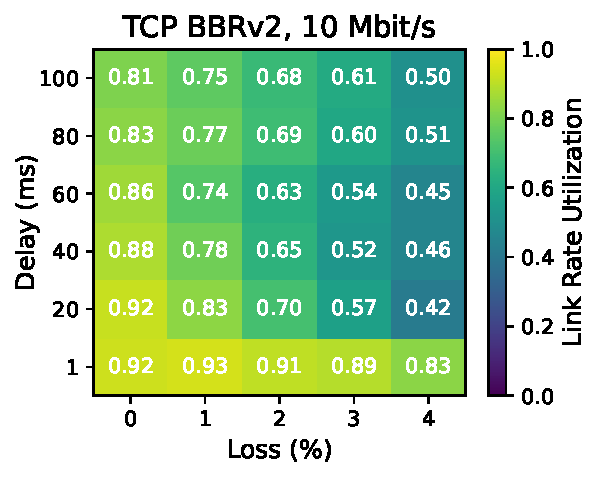
\includegraphics[width=\linewidth,trim={0 0 2cm 0.7cm},clip]
         {splitting-paper/figures/heatmaps/heatmap_tcp_bbr2_10mbps.pdf}
        \captionsetup{skip=4pt}
        \caption{TCP BBRv2.}
        \label{fig:2d-heatmap:bbr2-10}
    \end{subfigure}
    \begin{subfigure}[b]{0.22\linewidth}
        \centering
        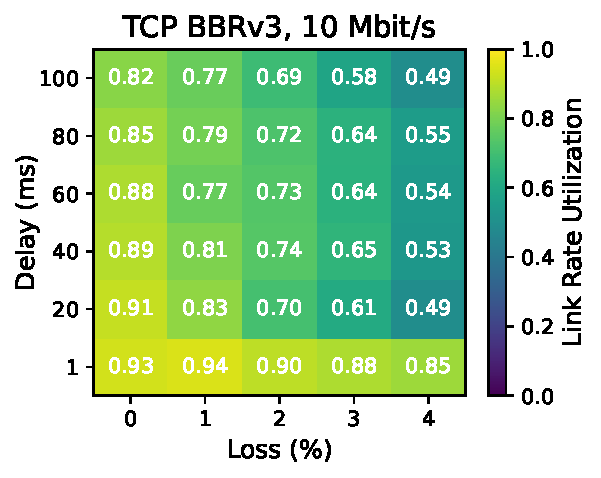
\includegraphics[width=\linewidth,trim={0 0 2cm 0.7cm},clip]
         {splitting-paper/figures/heatmaps/heatmap_tcp_bbr3_10mbps.pdf}
        \captionsetup{skip=4pt}
        \caption{TCP BBRv3.}
        \label{fig:2d-heatmap:bbr3-10}
    \end{subfigure}
    \begin{subfigure}[b]{1cm}
        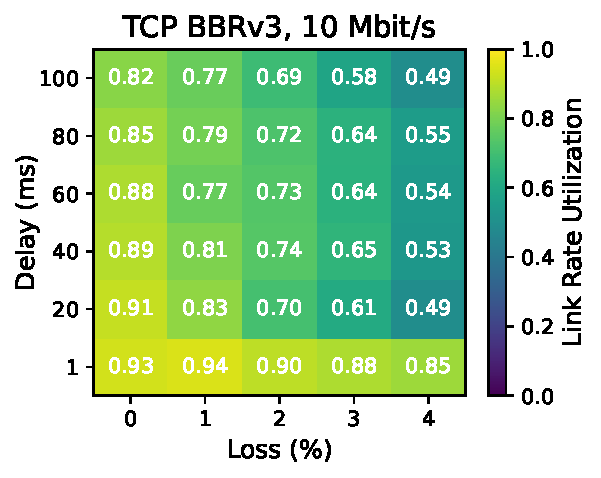
\includegraphics[width=1cm,trim={8cm 0 0 0},clip]
         {splitting-paper/figures/heatmaps/heatmap_tcp_bbr3_10mbps.pdf}
    \end{subfigure}
    \caption{The link rate utilization calculated as the ratio of achieved
     goodput to link rate for various TCP CCAs in an emulated network path, at
     various loss rates and one-way delays, at 10 Mbit/s. CUBIC is the
     most sensitive to loss and delay, while BBRv1 is the most aggressive and
     achieves the highest utilizations; BBRv2 and BBRv3 are more sensitive to
     loss than BBRv1 and utilization starts to suffer (left to right). CCAs
     tend to achieve lower utilizations, though higher absolute goodputs, as
     the link rate increases (\Cref{sec:appendix}). Median of $n=20$ trials.}
    \label{fig:2d-heatmap}
\end{figure*}


In our emulation measurement study, we aim to answer three questions to gain a
more comprehensive understanding of the relevance of connection-splitting with
modern networks:

\begin{enumerate}[noitemsep]
    \item Has the model-based BBR algorithm made the throughput enhancements of
     connection-splitting obsolete?
    \item Are there classes of network settings where BBR benefits significantly
     from splitting but CUBIC does not?
    \item How does CCA implementation impact end-to-end behavior, and therefore split
     behavior?
\end{enumerate}

\noindent To recap our measurement methodology, we have a method for
 measuring the throughput of TCP connections in emulation both with and without a
 transparent PEP. We also have the ability to estimate throughput both with and
 without a generic connection splitter, for both TCP and QUIC, based on
 knowledge of the network model of each path segment, and the measured end-to-end
 throughput on each segment.

For our analysis, we cache measurements for the end-to-end network parameters
in \Cref{tab:parameters} and the congestion control schemes in \Cref
{tab:cca-implementations}. We also run experiments in the two-segment network topology
to validate some of these predictions. Raw data for the end-to-end
behavior of each CCA implementation are available in \Cref{sec:appendix}.
Our emulation benchmarks are also publicly available on GitHub: \url{https://github.com/StanfordSNR/connection-splitting}.

\subsection{Finding 1: TCP BBR Over Time}
\label{sec:splitting:results:finding1}

\paragraph{Finding: Splitting has become significantly more beneficial to TCP
 BBR since it was initially released in 2016.}

Has the model-based BBR algorithm made the throughput enhancements of
connection-splitting obsolete? We find this line of thought has some truth
with the initial release of TCP BBRv1 in 2016. But as the BBR algorithm has
evolved into BBRv2 in 2019 and now BBRv3 in 2023, it has also evolved to behave
more conventionally in the sense that it benefits from being split---just like
more traditional, loss-based congestion control schemes such as CUBIC.

\Cref{fig:bbr-over-time} shows three different network settings in which BBRv2
and BBRv3 show significant throughput gains from connection-splitting.
 When BBRv1 was released, its throughput both with and
 without the connection-splitter were roughly the same, and nearly achieved the
 bottleneck link rate. With BBRv2 and BBRv3, the end-to-end throughput
 drastically deteriorated, behaving more like CUBIC than BBRv1. However, the
 split throughput remained relatively high, suggesting that BBRv3 today would
 still benefit from connection-splitting.

\paragraph{Analysis.}
To explore why CUBIC and BBRv3 benefit from splitting but BBRv1 does not, we
analyze end-to-end throughputs of each CCA and apply the split throughput
heuristic (\Cref{fig:heuristic}). As described in \Cref{sec:splitting:heuristic},
this methodology allows us to study split settings by measuring the much smaller
parameter space of end-to-end connections. We find that connection-splitting is
likely to improve throughput on lossy paths for CUBIC, BBRv2, and BBRv3
connections, but not for BBRv1.

\Cref{fig:2d-heatmap} visualizes our cached end-to-end measurements as link rate
 utilization heatmaps of loss vs. delay.
 Here is an example for how to interpret these graphs using \Cref
 {fig:2d-heatmap:bbr3-10}. The top-left cell represents a 100 ms 0\% segment
 with 0.82 utilization of the 10 Mbit/s link rate, and the bottom-right cell
 represents a 1 ms 4\% segment with 0.85 utilization of the 10 Mbit/s link
 rate. The predicted split utilization of a network path composed of these two
 segments is just 0.82, the minimum. The two cells compose to the top-right
 cell, which represents a 100 ms 4\% 10 Mbit/s segment with an end-to-end
 utilization of 0.49. Since $0.82>0.49$, we say that splitting has improved the
 throughput of this network path.

BBRv1 achieves high link rate utilization in all settings (\Cref
{fig:2d-heatmap:bbr1-10}), showing it has little to gain from splitting.
In fact, previous studies have shown that BBRv1 achieves $\approx\!85\%$
link utilization regardless of loss (same as our findings) before it reaches
a cliff point at around 20\% loss~\cite{cao2019use,cardwell2017bbr}.
This may be why it appears that splitting in lossy settings is now obsolete with BBR.
However, one should note that BBRv1's high throughput has long been attributed
to its aggressiveness and unfairness to legacy algorithms~\cite
{ware2019modeling,cao2019use}, which is what led to the changes in BBRv2 and
BBRv3.

While BBRv2 is a large departure from BBRv1, BBRv3 has been described as BBRv2
with bugfixes and performance tuning~\cite{cardwell2024bbrv3-ietf119}, which
supports why the two are so similar. We focus on BBRv3 since Google hopes to
now deprecate BBRv2~\cite{cardwell2024bbrv3-ietf119}.

BBRv3 is more sensitive to loss than its previous versions (\Cref
{fig:2d-heatmap:bbr3-10}), and more similar to CUBIC (\Cref
{fig:2d-heatmap:cubic-10}) in that there exist scenarios where end-to-end
throughput suffers.
These reflect existing findings of lower utilization in BBRv2 and BBRv3~\cite
{datta2023replication,song2021understanding,zeynali2024promises}.
Based on the heuristic, it is clear that in some lossy networks
such as the ones empirically evaluated in \Cref{fig:bbr-over-time},
connection-splitting
can significantly increase the throughput of BBRv3 connections.
It is possible that the BBR algorithm continues to evolve in this direction
given that BBR's unfairness remains contentious today~\cite
{datta2023replication,zeynali2024promises}.

\paragraph{Summary.}

While BBR may not have benefited from splitting with the release of ``v1'' in 2016, BBRv2 and
now BBRv3 have evolved to behave more conventionally---similar to traditional,
loss-based CCAs such as CUBIC---in the sense that they \textit{do}. Even
so-called ``model-based'' congestion control algorithms seem to now react to
loss as a congestion signal, as the BBR algorithm continues to evolve.

\subsection{Finding 2: TCP BBRv3 vs. TCP CUBIC}
\label{sec:splitting:results:finding2}

\paragraph{Finding: There exist classes of network paths where TCP BBRv3 would
 significantly benefit from splitting but TCP CUBIC would not.}

Are there new classes of network settings where BBR benefits significantly from
splitting but CUBIC does not? We want to understand the network settings in
which a congestion control scheme is not able to achieve practical bottleneck
link rate utilizations end-to-end, but is with a connection-splitter.

We find that while splitting benefits BBRv3 in all the same scenarios as CUBIC,
it also has the potential to benefit BBRv3 in many \textit{new} scenarios.
In addition to edge deployments with a lossy last-mile, BBRv3
also benefits from splitting in scenarios where there is loss on both path
segments, and when the connection-splitter is located farther from the edge.
We partition these scenarios into three classes of network settings:

\begin{enumerate}[label=\Roman*.,noitemsep]
\item Paths with asymmetric delay and a lossy last-mile,
\item Lossy paths with asymmetric delay,
\item Lossy paths with more symmetric delay.
\end{enumerate}

\noindent \Cref
 {fig:bbr-over-time:class1,fig:bbr-over-time:class2,fig:bbr-over-time:class3}
represent network settings in each class, respectively.
``Asymmetric'' refers to the delays on the two path segments.
These emulations empirically demonstrate that CUBIC only benefits in the first
class, while BBRv3 benefits in all three.
BBRv1 does not need splitting in any context.

\paragraph{Analysis.}
To identify which network paths benefit from connection-splitting and where
along the paths PEPs should be deployed, we apply the
heuristic (\Cref{fig:heuristic}).
For each CCA, we conduct an exhaustive search of the $15 \cdot 21 \cdot 25 =
7875$ combinations of settings within our parameter space (\Cref
{tab:parameters}), and efficiently predict the split and end-to-end throughputs.

We filter on the predicted throughputs for network settings where splitting improves end-to-end throughput by
at least $3\times$, and where the split connection utilizes at least half the
bottleneck link rate (\Cref{tab:network-path-analysis}). BBRv1 does not meet
these criteria is any scenarios, and the theoretical connection-splitter is
unable to improve the throughput of BBRv1 by even $50\%$. CUBIC and BBRv3 meet
these criteria in 942 and 188 scenarios, respectively. CUBIC benefits from
splitting in more scenarios because its end-to-end utilization is more
frequently low, so it more frequently has a large split improvement.

\begin{table}[t!]
  \centering
\begin{tabular}{ r l l l }
  \toprule
    \textbf{Filter} & \textbf{BBRv1} & \textbf{CUBIC} & \textbf{BBRv3} \\
    \midrule
    Initial & 7875 & 7875 & 7875 \\
    Split imprvmnt. $>3\times$ & 0 & 2231 & 234 \\
    Split utilization $>0.5$ & 0 & 942 & 188 \\
    \midrule
    Asymmetric, last-mile & 0 & 942 & 38 \\
    Asymmetric, lossy & 0 & 0 & 72 \\
    Symmetric, lossy & 0 & 0 & 78 \\
    \bottomrule
\end{tabular}
  \caption{\label{tab:network-path-analysis} An exhaustive search of network
   paths and their PEP locations that benefit from splitting for each CCA, and
   the number of filtered settings that belong to each class.}
  \vspace{-0.4cm}
\end{table}


Since the distribution of network paths in our parameter space does not reflect
any meaningful real world distribution, we are more interested in the \textit
{classes} of network settings that benefit from splitting. We realized
that \textit{all} of the relevant network settings for CUBIC can be clustered
into Class I, as network paths where one path segment has $1$ ms delay and
non-zero loss, and the other has $>1$ ms delay and $0\%$ loss. However, Class
I only accounts for $21\%$ of the relevant network settings for BBRv3. We
identify Class II, which is the same as I, except both path segments have
non-zero loss. Class III is the same as II, except both path segments have
$>1$ ms delay. We used the results to select three representative network
settings to empirically evaluate in \Cref{fig:bbr-over-time}.

Intuitively, we can understand why BBRv3 benefits more from splitting in lossy
scenarios than CUBIC based on how it reacts to loss and delay (\Cref
{fig:2d-heatmap:bbr3-10}). BBRv3's sensitivity to loss
and delay is more gradual than abrupt, so it is more likely to benefit when
splitting a lossy, high-delay network path in any way. In comparison, CUBIC's
throughput falls off a cliff for many of these segmentations.

\paragraph{Discussion.}
Do these results reflect where PEP deployments have been useful in the real
world? Connection-splitters have traditionally been found in satellite,
cellular, and Wi-Fi networks with a wireless link or rate policer~\cite
{edeline2019bottomup,honda2011still}. This resembles Class I, where the
network path consists of a lossy last-mile, and a reliable Internet path
segment. It makes sense then for PEPs to be traditionally located at the edge
to address the issues of loss-based schemes~\cite
{cloudsplitting2010,rfc3135,farkas2012splittcp}. We expect these PEPs to
similarly benefit BBRv3 in the same locations.

In Classes I and II, asymmetric delay can be severe in low-resource networks
in addition to wireless last-mile links;
Consider, for example, regions with no IXPs in which a significant proportion
of Internet traffic travels internationally.

For Classes II and III, satellite (and also wireless ad-hoc)
networks are known for
having lossy ``middle-miles''~\cite{kuhn2021quic-over-sat,border2020evaluating,pirovano2013new,cloudsplitting2010}.
This can be due to bad weather, fast-moving satellites, and
long-distance radio waves, etc.
Since CUBIC does not trivially benefit from splitting in these scenarios, the
traditional solution has been to split the connection at multiple points and to
use an FEC-based or other proprietary protocol in the satellite backhaul~\cite
{cloudsplitting2010,border2020evaluating,rfc3135}.
Our results suggest such an invasive solution may not be necessary for BBRv3.

How could this inform the deployment of connection-splitting PEPs?
With the caveat that futher exploration is required to understand how the
heuristic extrapolates to the real world, one idea is to
determine where to deploy PEPs along an existing network path for maximum
benefit especially as congestion-control schemes evolve.
Another idea is given the location of a PEP, determine which connections going
through the PEP would most benefit based on knowledge of each connection's
network path.
We leave network operators to decide how best to model their networks and apply
the heuristic to evaluate potential PEP deployments.

\paragraph{Summary.}
While TCP CUBIC only benefits from connection-splitting when the PEP is located
at the lossy last-mile, TCP BBRv3 can also benefit when there is loss on both
sides of the PEP and when there are longer propagation delays. This suggests
that TCP connections using BBRv3 should benefit from splitters at the same
locations as for CUBIC, and also that traditional methods used to
address loss in the middle-mile could use simple connection-splitting instead.
We believe this method of analyzing useful network paths and PEP placements for
connection-splitting can be extended to model new types of networks, especially
in space.

\subsection{Finding 3: QUIC Congestion Control}
\label{sec:splitting:results:finding3}

\paragraph{Finding: QUIC implementations of the same congestion control schemes
 vary significantly, and further differ from Linux's TCP implementations.}

\begin{figure*}[t!]
    \centering
    \begin{subfigure}[b]{0.22\linewidth}
        \centering
        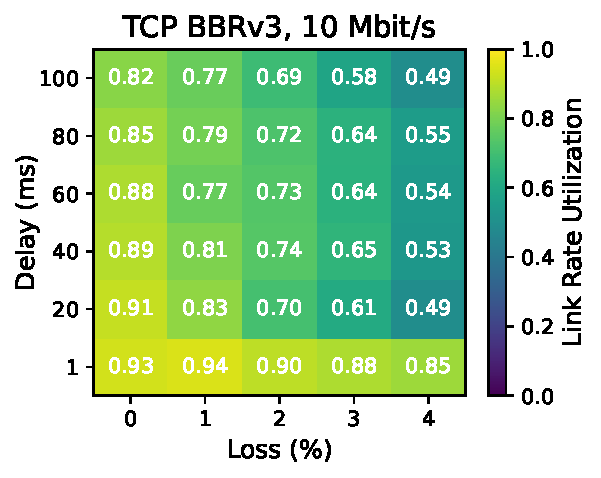
\includegraphics[width=\linewidth,trim={0 0 2cm 0.7cm},clip]
        {splitting-paper/figures/heatmaps/heatmap_tcp_bbr3_10mbps.pdf}
        \captionsetup{skip=4pt}
        \caption{TCP, BBRv3}
        \label{fig:quic:tcp-bbr3}
    \end{subfigure}
    \begin{subfigure}[b]{0.22\linewidth}
        \centering
        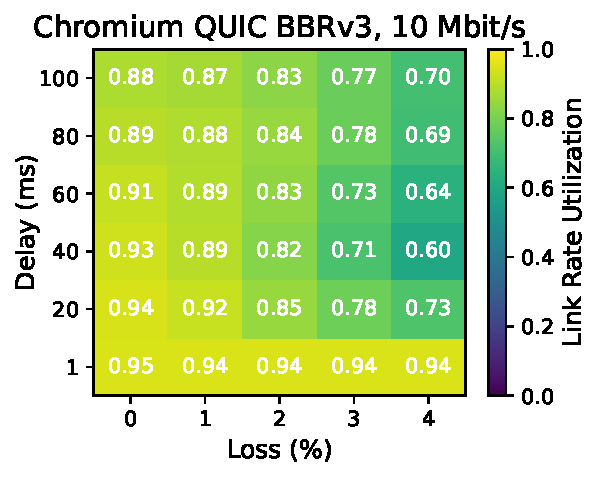
\includegraphics[width=\linewidth,trim={0 0 2cm 0.7cm},clip]
        {splitting-paper/figures/heatmaps/heatmap_quic_bbr3_10mbps.pdf}
        \captionsetup{skip=4pt}
        \caption{Google \texttt{quiche}, BBRv3}
        \label{fig:quic:google-bbr3}
    \end{subfigure}
    \begin{subfigure}[b]{0.22\linewidth}
        \centering
        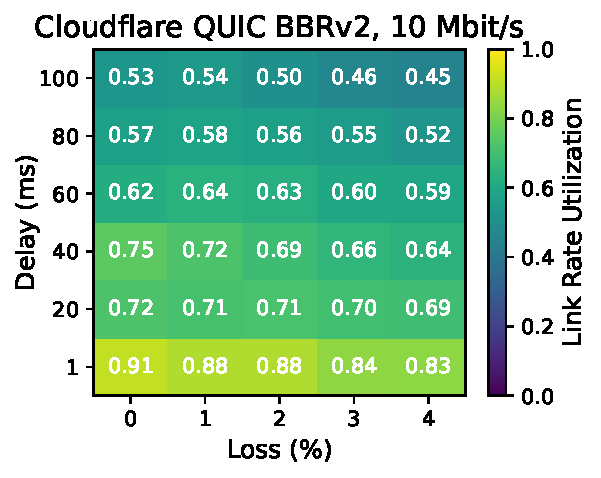
\includegraphics[width=\linewidth,trim={0 0 2cm 0.7cm},clip]
        {splitting-paper/figures/heatmaps/heatmap_quiche_bbr2_10mbps.pdf}
        \captionsetup{skip=4pt}
        \caption{Cloudflare \texttt{quiche}, BBRv2}
        \label{fig:quic:cloudflare-bbr2}
    \end{subfigure}
    \begin{subfigure}[b]{0.22\linewidth}
        \centering
        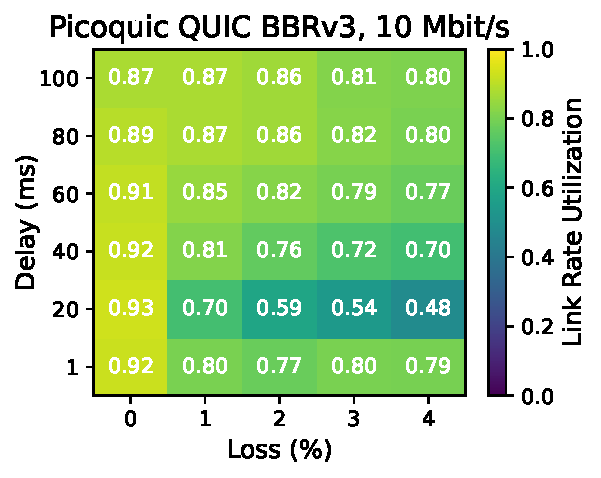
\includegraphics[width=\linewidth,trim={0 0 2cm 0.7cm},clip]
        {splitting-paper/figures/heatmaps/heatmap_picoquic_bbr3_10mbps.pdf}
        \captionsetup{skip=4pt}
        \caption{\texttt{picoquic}, BBRv3}
        \label{fig:quic:picoquic-bbr3}
    \end{subfigure}
    \begin{subfigure}[b]{1cm}
        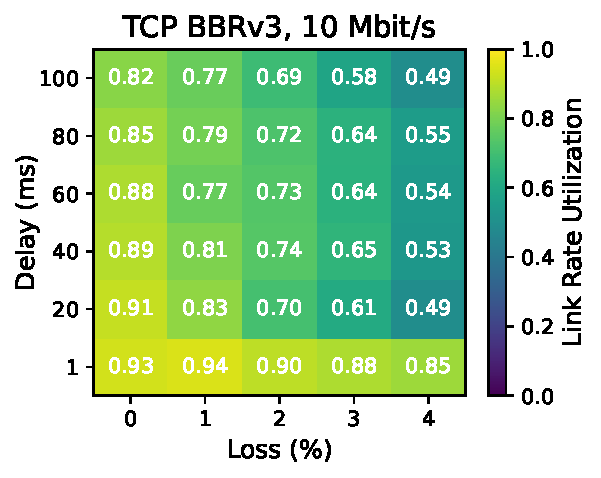
\includegraphics[width=1cm,trim={8cm 0 0 0},clip]
        {splitting-paper/figures/heatmaps/heatmap_tcp_bbr3_10mbps.pdf}
        \vspace*{0.2cm}
    \end{subfigure}
    
    \begin{subfigure}[b]{0.22\linewidth}
        \centering
        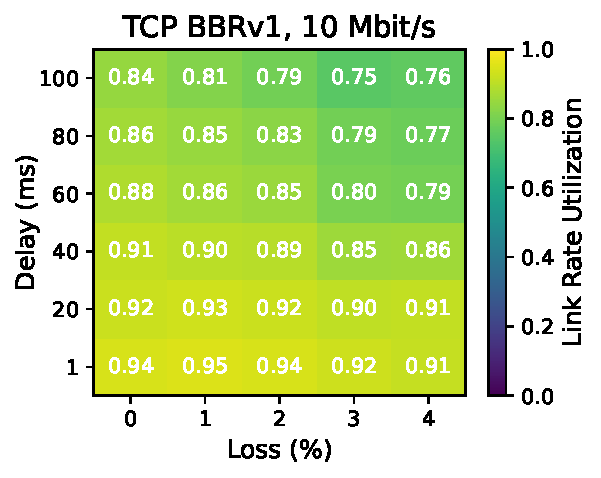
\includegraphics[width=\linewidth,trim={0 0 2cm 0.7cm},clip]
        {splitting-paper/figures/heatmaps/heatmap_tcp_bbr1_10mbps.pdf}
        \captionsetup{skip=4pt}
        \caption{TCP, BBRv1}
        \label{fig:quic:tcp-bbr1}
    \end{subfigure}
    \begin{subfigure}[b]{0.22\linewidth}
        \centering
        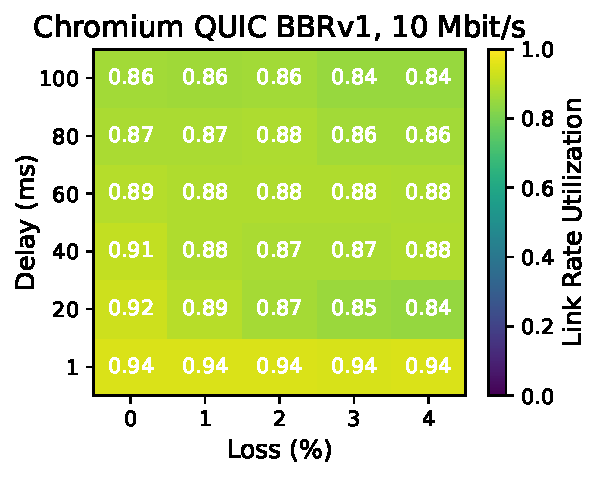
\includegraphics[width=\linewidth,trim={0 0 2cm 0.7cm},clip]
        {splitting-paper/figures/heatmaps/heatmap_quic_bbr1_10mbps.pdf}
        \captionsetup{skip=4pt}
        \caption{Google \texttt{quiche}, BBRv1}
        \label{fig:quic:google-bbr1}
    \end{subfigure}
    \begin{subfigure}[b]{0.22\linewidth}
        \centering
        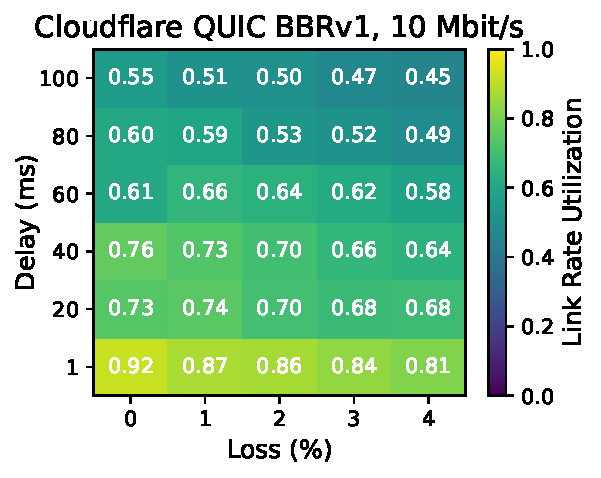
\includegraphics[width=\linewidth,trim={0 0 2cm 0.7cm},clip]
        {splitting-paper/figures/heatmaps/heatmap_quiche_bbr1_10mbps.pdf}
        \captionsetup{skip=4pt}
        \caption{Cloudflare \texttt{quiche}, BBRv1}
        \label{fig:quic:cloudflare-bbr1}
    \end{subfigure}
    \begin{subfigure}[b]{0.22\linewidth}
        \centering
        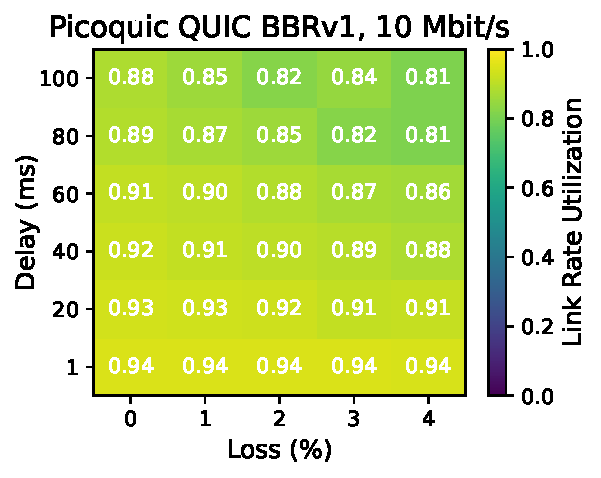
\includegraphics[width=\linewidth,trim={0 0 2cm 0.7cm},clip]
        {splitting-paper/figures/heatmaps/heatmap_picoquic_bbr1_10mbps.pdf}
        \captionsetup{skip=4pt}
        \caption{\texttt{picoquic}, BBRv1}
        \label{fig:quic:picoquic-bbr1}
    \end{subfigure}
    \begin{subfigure}[b]{1cm}
        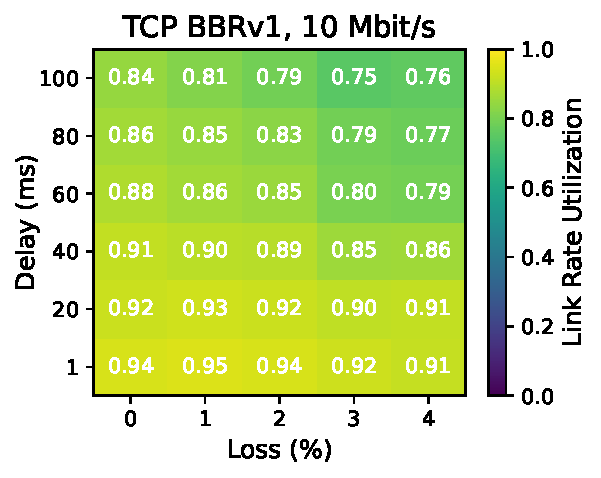
\includegraphics[width=1cm,trim={8cm 0 0 0},clip]
        {splitting-paper/figures/heatmaps/heatmap_tcp_bbr1_10mbps.pdf}
        \vspace*{0.2cm}
    \end{subfigure}

    \begin{subfigure}[b]{0.22\linewidth}
        \centering
        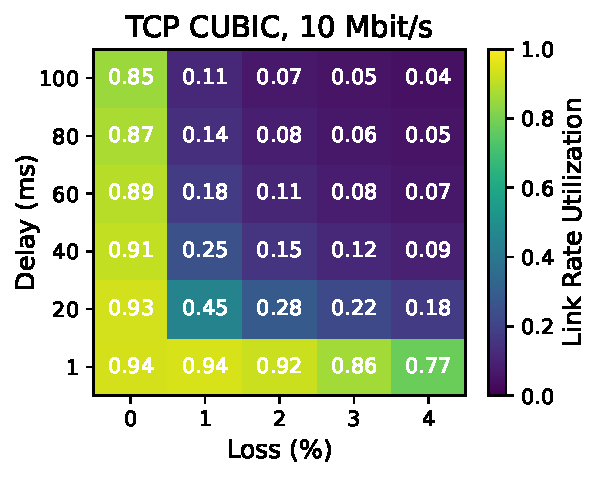
\includegraphics[width=\linewidth,trim={0 0 2cm 0.7cm},clip]
        {splitting-paper/figures/heatmaps/heatmap_tcp_cubic_10mbps.pdf}
        \captionsetup{skip=4pt}
        \caption{TCP, CUBIC}
        \label{fig:quic:tcp-cubic}
    \end{subfigure}
    \begin{subfigure}[b]{0.22\linewidth}
        \centering
        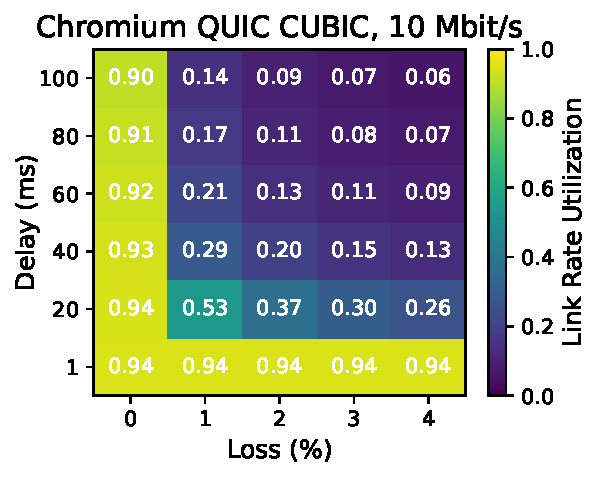
\includegraphics[width=\linewidth,trim={0 0 2cm 0.7cm},clip]
        {splitting-paper/figures/heatmaps/heatmap_quic_cubic_10mbps.pdf}
        \captionsetup{skip=4pt}
        \caption{Google \texttt{quiche}, CUBIC}
        \label{fig:quic:google-cubic}
    \end{subfigure}
    \begin{subfigure}[b]{0.22\linewidth}
        \centering
        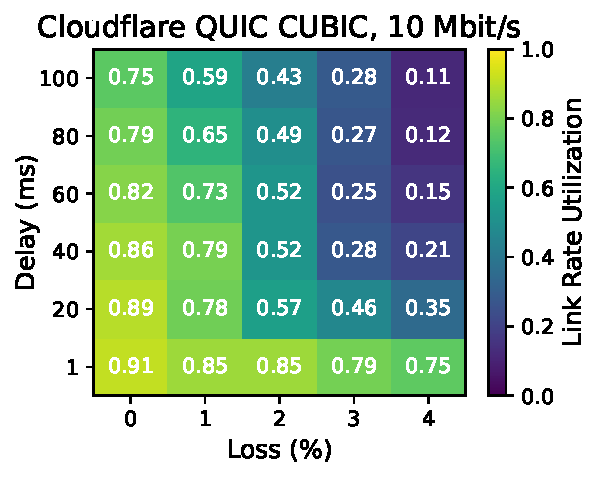
\includegraphics[width=\linewidth,trim={0 0 2cm 0.7cm},clip]
        {splitting-paper/figures/heatmaps/heatmap_quiche_cubic_10mbps.pdf}
        \captionsetup{skip=4pt}
        \caption{Cloudflare \texttt{quiche}, CUBIC}
        \label{fig:quic:cloudflare-cubic}
    \end{subfigure}
    \begin{subfigure}[b]{0.22\linewidth}
        \centering
        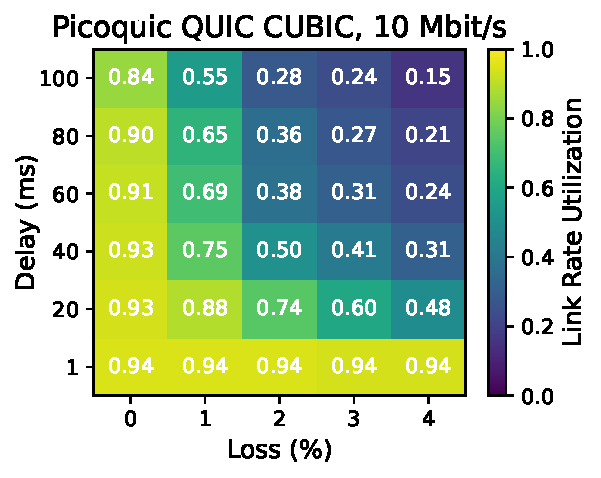
\includegraphics[width=\linewidth,trim={0 0 2cm 0.7cm},clip]
        {splitting-paper/figures/heatmaps/heatmap_picoquic_cubic_10mbps.pdf}
        \captionsetup{skip=4pt}
        \caption{\texttt{picoquic}, CUBIC}
        \label{fig:quic:picoquic-cubic}
    \end{subfigure}
    \begin{subfigure}[b]{1cm}
        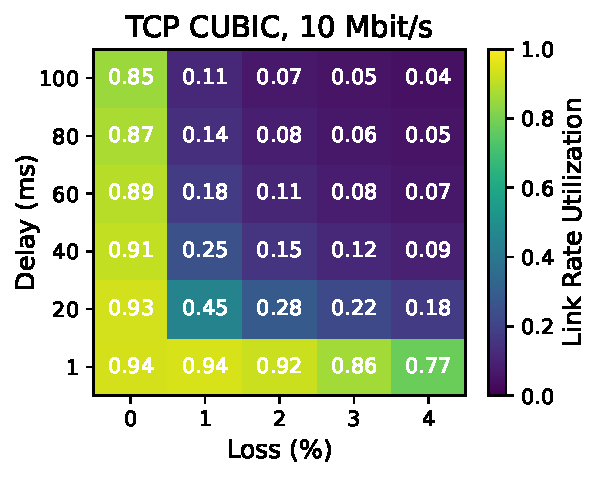
\includegraphics[width=1cm,trim={8cm 0 0 0},clip]
        {splitting-paper/figures/heatmaps/heatmap_tcp_cubic_10mbps.pdf}
        \vspace*{0.2cm}
    \end{subfigure}

    \caption{Heatmaps for three QUIC implementations of BBRv3 (or BBRv2), BBRv1,
     and CUBIC showing link rate utilization calculated as the ratio of
     achieved goodput to link rate, compared to Linux TCP. The heatmaps are
     shown at various loss rates and one-way delays with a fixed link rate of
     10 Mbit/s. User-space QUIC is not CPU-limited, achieving high utilizations
     at 1 ms delay and 0\% loss. The QUIC implementations are Google \texttt
     {quiche}, Cloudflare \texttt{quiche}, and a minimalist implementation
     based on the IETF spec called \texttt{picoquic}. Median of $n=20$
     trials.}
    \label{fig:quic}
    \vspace{-0.3cm}
\end{figure*}


How does CCA implementation impact end-to-end behavior, and therefore split
behavior? Might claims about ``split throughput'' depend not just on the CCA,
but also the \textit{implementation} and/or the transport protocol
on top of it?

For our initial study, we compared end-to-end throughput for four open-source
implementations each of CUBIC, BBRv1, and BBRv2/3; one using TCP and three
using QUIC. We find that the end-to-end behavior of each CCA varies by
implementation in both baseline throughput and sensitivity to loss and delay.
To evaluate the split behavior of QUIC, instead of creating a custom and
explicit connection-splitting PEP for each QUIC implementation, we apply the
split throughput heuristic and argue that these implementations
will likewise respond differently to connection-splitting PEPs.

\Cref{fig:quic} visualizes the end-to-end behavior of these schemes.
We highlight that the Cloudflare and \texttt
 {picoquic} CUBIC implementations are less sensitive to loss than Google or
 TCP; the former may benefit from splitting in more classes of network settings
 than the latter. Additionally, their BBR implementations exhibit non-uniform
 behavior, suggesting a non-uniform response to
 connection-splitting. These variations indicate that the benefits of
 in-network assistance should be considered along with not just the CCA but its
 specific implementations.

\paragraph{Analysis.}

The Google QUIC (\Cref{fig:quic:google-bbr1,fig:quic:google-bbr3,fig:quic:google-cubic})
and TCP (\Cref{fig:quic:tcp-bbr1,fig:quic:tcp-bbr3,fig:quic:tcp-cubic})
implementations are most similar to each other for each CCA.
This is reasonable if we take the community-based CUBIC implementation in
Linux to be the standard, and considering that Google contributed to the Linux
BBR implementations. In general, Google QUIC achieves slightly higher
utilization than Linux TCP.

The Cloudflare QUIC BBR implementations (\Cref{fig:quic:cloudflare-bbr1,fig:quic:cloudflare-bbr2})
exhibit profoundly different behavior from Linux TCP in baseline performance.
Note that Cloudflare uses BBRv1 for TCP but their use of BBR in QUIC
is experimental. Anecdotally, a
Cloudflare employee has expressed difficulty making
their BBR implementation performant, having to reverse engineer
the Linux kernel~\cite{cardwell2024bbrv3-ietf119-qna}. Given the wide adoption
of BBRv1 for TCP at many CDNs~\cite{ware2024ccanalyzer}, we expect it to
be desirable yet challenging for these same companies to correctly incorporate
BBRv3 into their QUIC stacks in the coming years.
% Maybe cite narayan2018restructuring

The \texttt{picoquic} BBR implementations (\Cref{fig:quic:picoquic-bbr1,fig:quic:picoquic-bbr3})
are more similar to Linux TCP, although its BBRv3 implementation seems to have
a contradicting reaction to delay.
We note that \texttt{picoquic} is intended for experimental use in the
IETF~\cite{picoquic}. It is important then to understand its congestion control
behavior if it is to be used to evaluate
IETF proposals. We believe its differences from Linux TCP warrant further
exploration, but perhaps also that the ongoing standardization efforts of BBR
in the IETF~\cite{cardwell2024bbr-ietf-draft} indicate
that there is no monolith yet of ``the BBR algorithm.''

The Cloudflare QUIC and \texttt{picoquic} implementations of CUBIC
(\Cref{fig:quic:cloudflare-cubic,fig:quic:picoquic-cubic}) interestingly
both exhibit a more gradual degradation in response to loss and delay than Linux TCP
(\Cref{fig:quic:tcp-cubic}). We
find this harder to explain, given that TCP CUBIC has been around since 2006,
and perhaps can be attributed to transport protocol mechanisms in QUIC.
Nevertheless, this indicates that it is important to understand the
behavior of a CCA in the context of its entire
implementation.

\begin{figure}[t!]
    \centering
    \begin{subfigure}[b]{\linewidth}
        \centering
        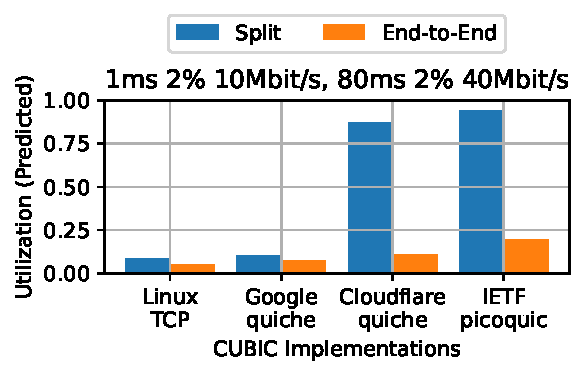
\includegraphics[width=0.8\linewidth]
         {splitting-paper/figures/network_path_analysis/network_path_analysis_10_40_1_80_2_2.pdf}
        \captionsetup{skip=0pt}
        \caption{Some QUIC CUBIC implementations can benefit in new network
         classes where TCP CUBIC could not.}
        \label{fig:quic-predictions:cubic}
    \end{subfigure}
    \begin{subfigure}[b]{\linewidth}
        \centering
        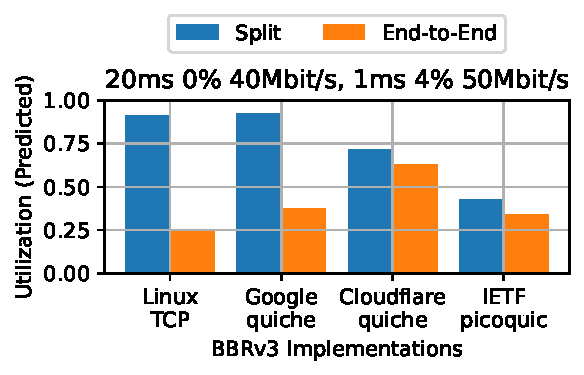
\includegraphics[width=0.8\linewidth]
         {splitting-paper/figures/network_path_analysis/network_path_analysis_40_50_20_1_0_4.pdf}
        \captionsetup{skip=0pt}
        \caption{The various BBRv3 implementations have non-uniform end-to-end
         behavior and no clear resulting split behavior.}
        \label{fig:quic-predictions:bbr3}
    \end{subfigure}
    \caption{Predicted bottleneck link rate utilizations calculated from the
     predicted end-to-end and split throughputs of the TCP and QUIC
     implementations, on two different network path segments. End-to-end
     behavior of each CCA varies significantly by implementation.}
    \label{fig:quic-predictions}
\end{figure}


\Cref{fig:quic-predictions} applies the heuristic to show how split behavior
can vary for CCA implementations with different end-to-end behaviors.
Some QUIC CUBIC implementations
benefit in new network settings where TCP CUBIC does not, while the various
QUIC BBRv3 implementations exhibit non-uniform end-to-end behavior and thus no
clear trend in split behavior.

\paragraph{Discussion.}

Why do we believe we can extrapolate split behavior from the end-to-end behavior
of QUIC? Previous studies explore the effects of QUIC's transport protocol
mechanisms in such a case~\cite{kosek2022quicpep,thomas2019google}. They find
that the effects of zero-RTT connection establishment with regards to
long-lived throughput to be minimal, and stream multiplexing to be mutually
beneficial in both scenarios. Further studies can clarify the interactions
between CCAs and transport mechanisms.

How do we know that the difference in behavior is due to the congestion control
implementation and not other transport protocol mechanisms? Well, we
don't, and there is known to be significant variance in the features supported
by different QUIC implementations~\cite{marx2020same}.
However, we find it intuitive that congestion control would be a major factor in
the measured sustained goodput of a bulk file transfer.

The divergence in QUIC implementations is not so dissimilar from that of TCP at
a similar state of evolution~\cite{allman1999effective}, but there are still
some fundamental differences. With QUIC implementations in userspace, there is
a larger diversity of implementations that are easier to tune for a specific
application metric, as opposed to correctness or fairness from a
congestion-control point of view. These algorithms are also highly
parameterized, with no standard nor test suite, so it's not surprising that the
implementations differ.

If there is reason to believe
that QUIC is losing out on throughput by not connection-splitting, then there
will continue to be research on how to achieve the same benefits without
ossification~\cite{kosek2023secure,yuan2024sidekick,kramer2021masquepep,yuan2022sidecar}.
The heuristic helps us understand the theoretical achievable
throughput with a simple connection-splitter, or even by combining multiple
end-to-end congestion control schemes.
In addition to research, this could motivate privacy-minded proposals in the Internet
standards community to also view themselves as potential deployment opportunities
for private PEPs~\cite{kosek2021masque,sattler2022towards,rfc9297,rfc9298}.

Another application of analyzing CCA implementations is to analyze the Linux TCP
implementations of BBR \textit{within} a major version over time. We did
this analysis with BBRv1 on 13 Linux kernels between 2016 and 2024, but found
no significant variance. However, given the dynamic nature of BBR and the
Linux networking stack, it
is possible there will still be changes to the split behavior of TCP in the future.

\paragraph{Summary.}

We believe it is important to understand the end-to-end behavior of a congestion
control scheme in the context of its entire implementation.
Our results suggest that BBR is challenging to implement, and that even CUBIC
implementations can vary based on context. Whether the prevailing wisdom is
that a specific CCA or transport protocol has made in-network assistance
undesirable, these results suggest that it is valuable to consistently
re-evaluate these claims.

\section{Accuracy Analysis}
\label{sec:splitting:accuracy}

\begin{figure*}[t]
    \centering
    \begin{subfigure}[b]{0.325\linewidth}
        \centering
        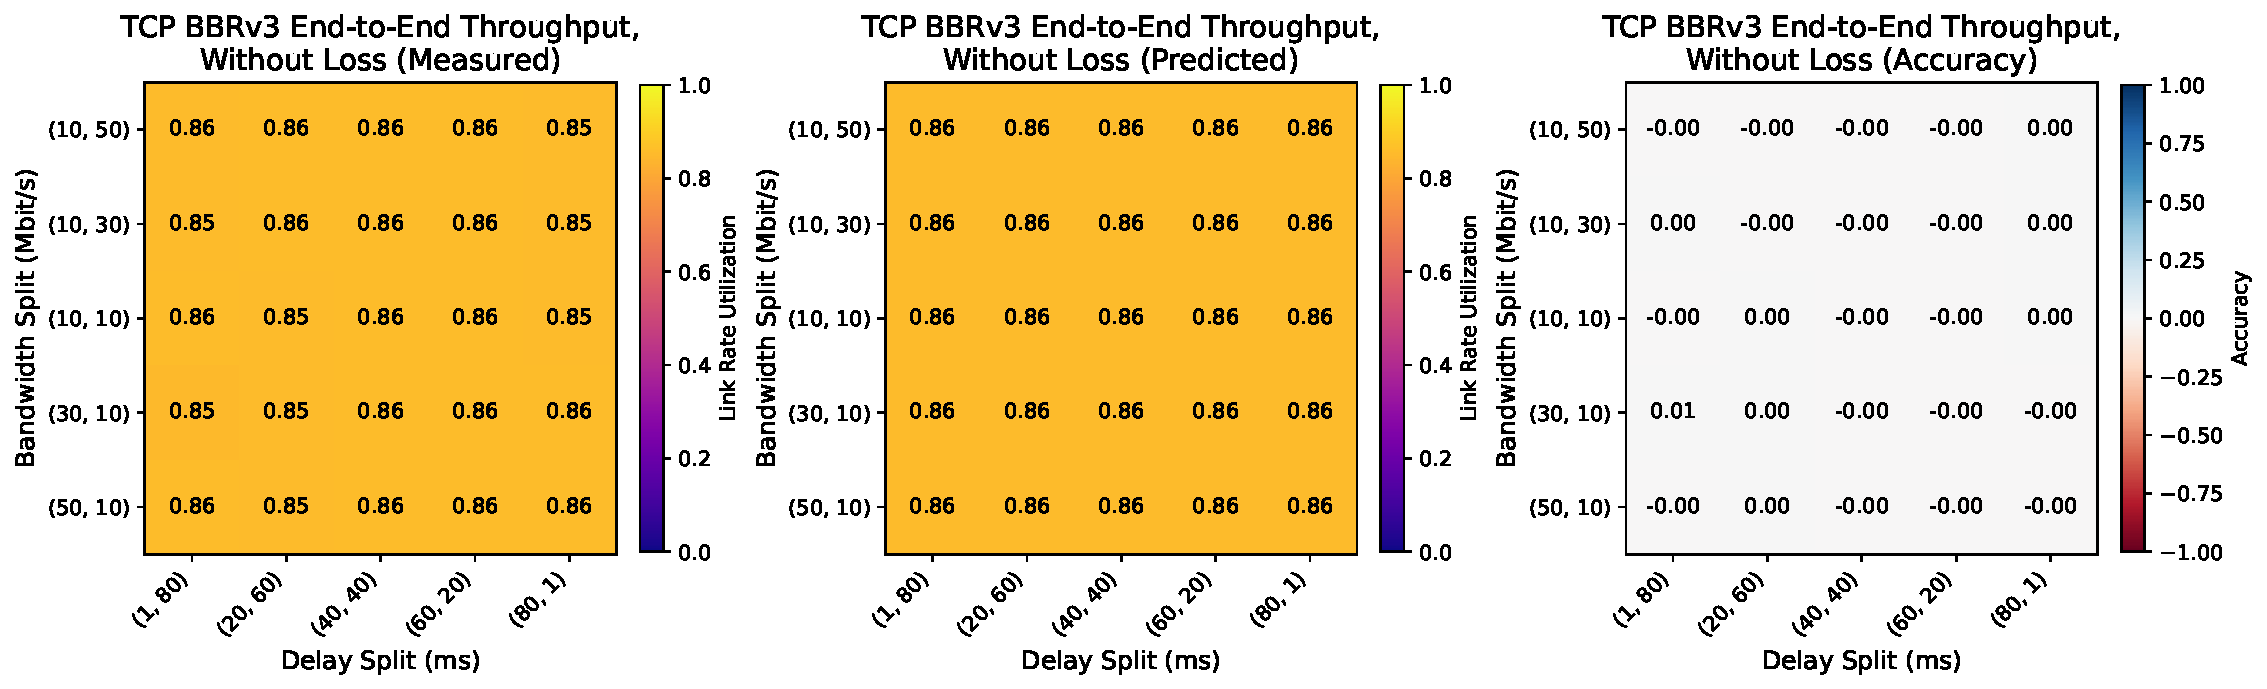
\includegraphics[width=\linewidth,trim={0 0 25.8cm 0},clip]
         {splitting-paper/figures/accuracy/accuracy_e2e_without_loss.pdf}
        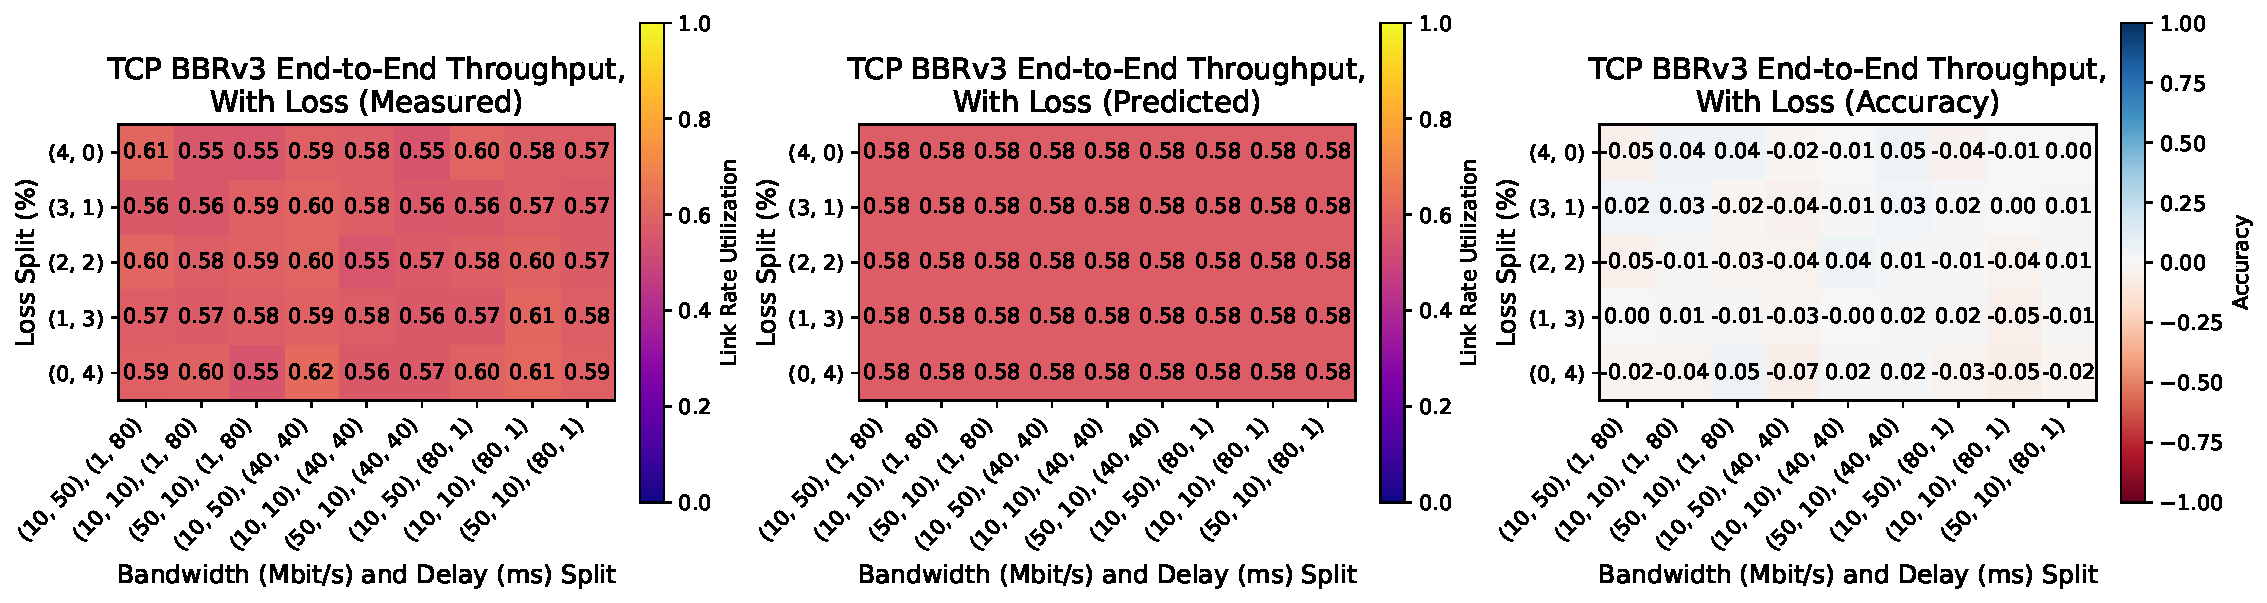
\includegraphics[width=\linewidth,trim={0 0 25.8cm 0},clip]
         {splitting-paper/figures/accuracy/accuracy_e2e_with_loss.pdf}
        \captionsetup{skip=4pt}
        \caption{End-to-end throughput accuracy.}
        \label{fig:accuracy:e2e}
    \end{subfigure}
    \begin{subfigure}[b]{0.645\linewidth}
        \centering
        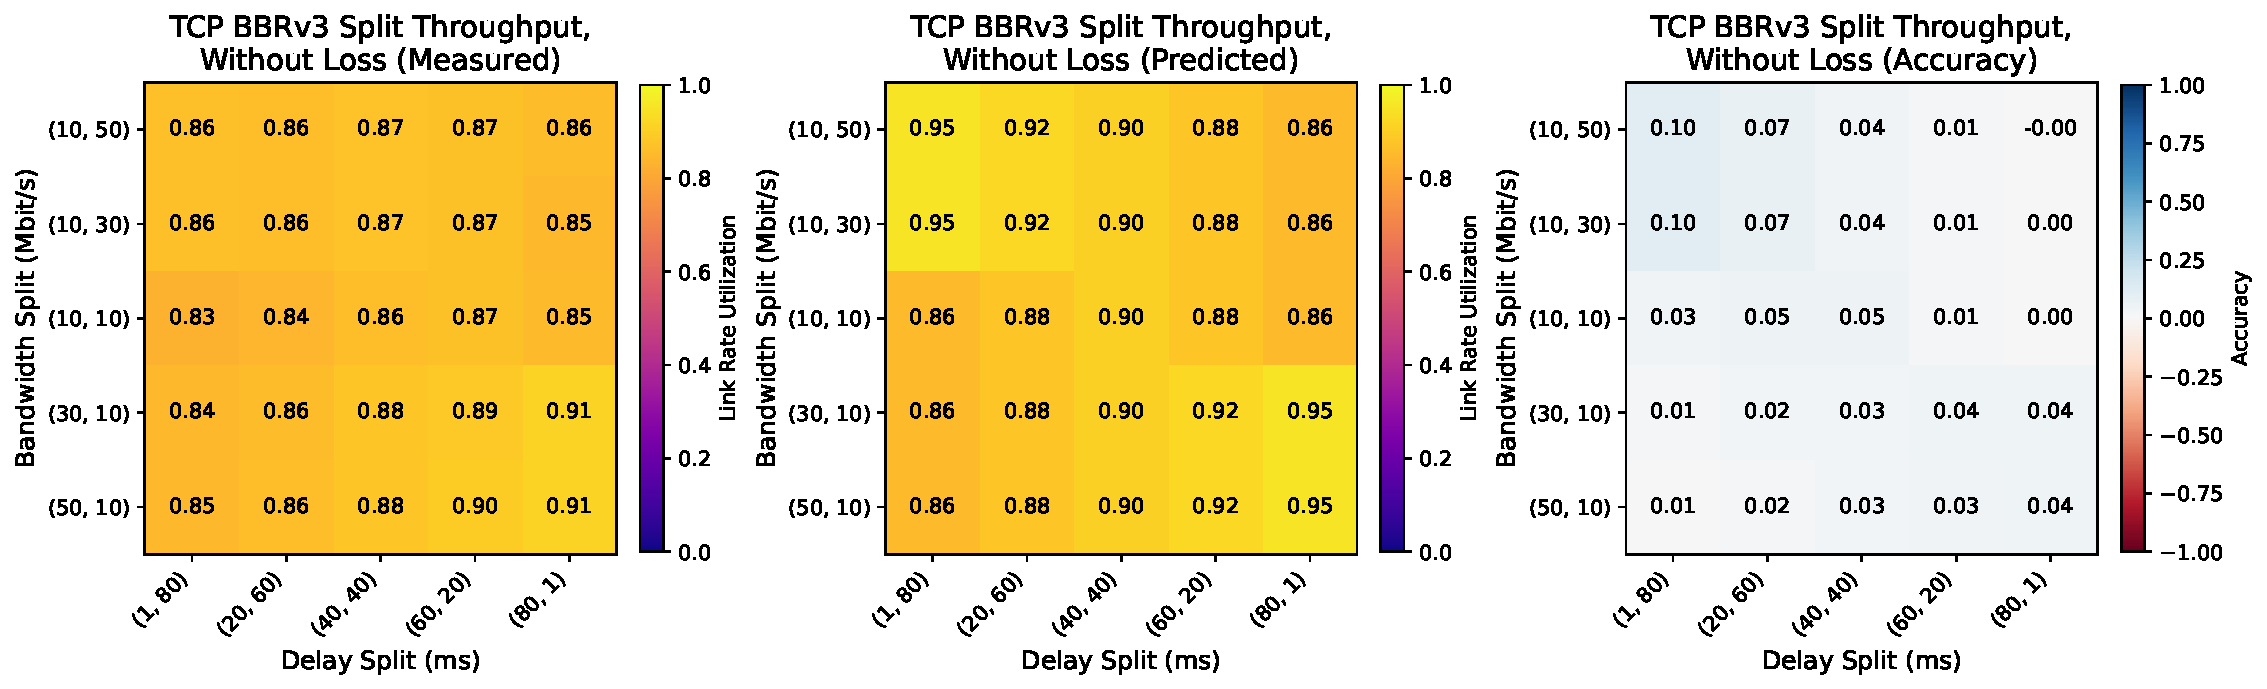
\includegraphics[width=\linewidth,trim={0 0 13.4cm 0},clip]
         {splitting-paper/figures/accuracy/accuracy_split_without_loss.pdf}
        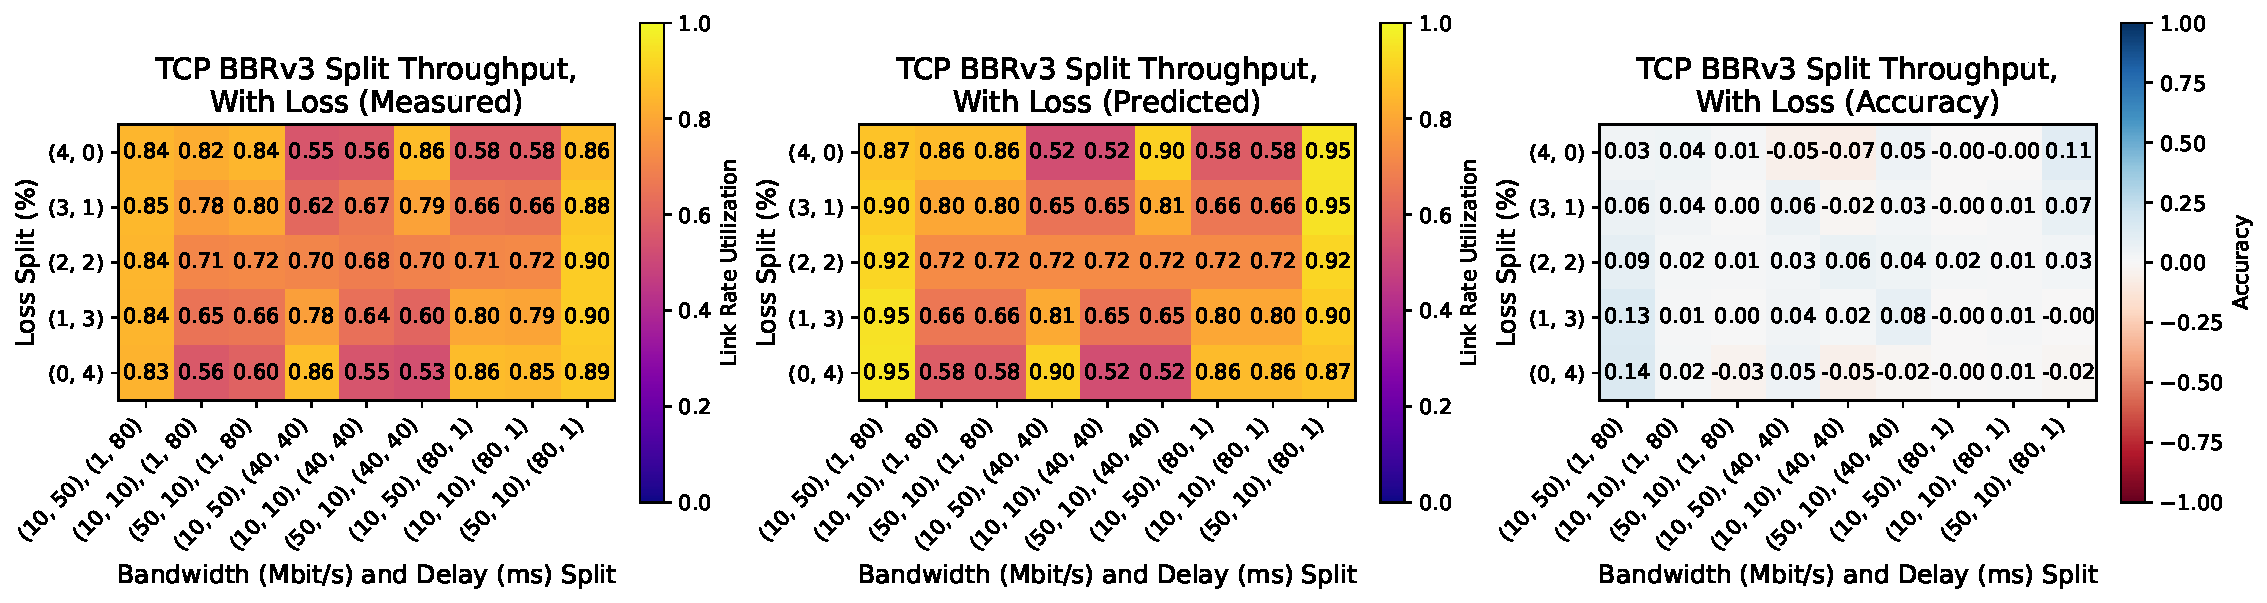
\includegraphics[width=\linewidth,trim={0 0 13.4cm 0},clip]
         {splitting-paper/figures/accuracy/accuracy_split_with_loss.pdf}
        \captionsetup{skip=4pt}
        \caption{Split throughput accuracy.}
        \label{fig:accuracy:split}
    \end{subfigure}

    \caption{Heatmaps of the measured and predicted BBRv3 throughputs for
     various splits of delay, bandwidth, and loss, both without (top) and with
     (bottom) loss.
     The \textit{end-to-end throughput} predictions (not pictured) are the same for all
     cells at 0.86 utilization without loss and 0.58 utilization with loss,
     because they represent the same network path, so end-to-end
     prediction errors are roughly uniform.
     The \textit{split throughput} predictions err slightly on the side of
     overestimation, but they accurately reflect trends in higher or lower throughputs for
     measurements on different splits of the same network path. Median of $n=40$ trials.}
    \label{fig:accuracy}
    \vspace{-0.3cm}
\end{figure*}


Our analysis of connection-splitting for TCP and its extensions to QUIC rely on
the accuracy of the split throughput heuristic. In this section, we are
primarily concerned with how accurate our predictions, which are based on
measurements from a one-segment topology, are for measurements from a
two-segment topology in emulation, without and with a connection-splitting TCP
PEP:
\begin{itemize}[noitemsep]
\item Does the \texttt{compose} function accurately represent the combined
 network path in the end-to-end throughput?
\item Does the split throughput heuristic accurately predict split throughput?
\end{itemize}

\noindent Most importantly, we find the heuristic to be able to usefully
 predict \textit{trends}.
 In terms of absolute predictions, we find the \texttt{pred\_e2e\_throughput()}
 and \texttt{pred\_split\_throughput()} functions to be correct within a
 reasonable tolerance, with a slight tendency to overestimate.

Orthogonally, we do not evaluate the accuracy to which emulation studies reflect
the real world with multi-flow settings and more complex network properties,
nor how the accuracy would extrapolate to QUIC connections with custom
connection splitters. It may be interesting to explore how to incorporate
such factors into the network model and heuristic.

\paragraph{Methodology.} Recall that for a given network path composed of two
 path segments, we can obtain both the predicted end-to-end and split
 throughputs, and the ground truth throughputs in an emulated network with and
 without a TCP PEP. Then for a network setting, we can compute the accuracy as
 the percent error in predicted vs. measured throughput.

We perform an empirical accuracy analysis of BBRv3 for two end-to-end network paths with
identical bandwidth and delay, both without (0\%) and with (4\%) loss. We test
various splits for the bandwidth, delay, and loss and analyze the accuracy
trends. In particular, we select delay splits such that the end-to-end delay is
80 ms, bandwidth splits such that the bottleneck bandwidth is 10 Mbit/s, and loss
splits such that the total loss is either 0\% or 4\%. We parameterize the network
path segments to use the cached measurements from \Cref
{tab:parameters}.

\paragraph{End-to-End Throughput Accuracy.}

Each of our splits composes to the same end-to-end network path, so we predict
the same end-to-end throughput for each. Our experimental
results in \Cref{fig:accuracy:e2e} show that the measured end-to-end
throughputs are also roughly uniform, especially without loss, indicating that
our method of composing network path segments in emulation represents the same
end-to-end network path.

\paragraph{Split Throughput Accuracy.}

The split throughput predictions accurately reflect trends in loss, delay, and
bandwidth (\Cref{fig:accuracy:split}). For example, split throughput is
generally higher when the high-bandwidth link is paired with high delay
(the yellow-est cells). It is also lower when the lossy link is paired with
high delay (columns 1 and 2) or low bandwidth (columns 3-5).

The split throughput predictions tend to slightly overestimate, but we think
the level of error is small enough to be helpful for informing real PEP
deployment. The maximum error is $\pm14\%$, and on average $\pm4\%$. This
dwarfs the measured gains in some situations, and rules out a large gain in
others.

One factor that may lead to overestimation of split throughput is the queue
behavior and the burstiness of the sender. With small queues and bursty
sending, we would expect the far path segment from the data sender to sometimes
be limited by the send buffer. This could subsequently affect how the far
connection probes for and utilizes available link rate capacity.

Another factor is the proximity of the bottleneck link to the sender. While
our heuristic does not account for this, the real split throughputs for
symmetric pairs of network paths (e.g., the left three and right three columns
in \Cref{fig:accuracy:split}), show that we slightly overestimate
when the low-bandwidth bottleneck link is far from the sender.
Based on our reasoning about queues, this would suggest that the far path
segment, already the bottleneck, is even further under-saturated.

Overall, we find our end-to-end and split throughput predictions to usefully
reflect relative trends and absolute throughput within a
reasonable tolerance. They are not intended to make claims about exact achievable
throughputs nor about the immediate utility of PEPs in the real world,
but simply to reason about how connection-splitting may impact
long-lived throughput in a simplified network model.
